% =============================================================================
% Copyright © 2026 Fredrik Bierich
% 
% This file is licensed under the Creative Commons Attribution-NonCommercial-
% ShareAlike 4.0 International License (CC BY-NC-SA 4.0).
%
% You are free to share and adapt this material for non-commercial purposes,
% provided you give appropriate credit and distribute your contributions under 
% the same license. Commercial use and sale are strictly prohibited.
%
% For commercial licensing inquiries, please contact: fredrik.bierich@gmail.com
% =============================================================================
\documentclass[a4paper,12pt]{report}
\usepackage{amsmath}
\usepackage{amssymb}
\usepackage[margin=1in]{geometry}
\usepackage{graphicx}
\usepackage{lmodern}
\usepackage{pdflscape}
\usepackage{subcaption}
\usepackage{tikz}
\usepackage{titlesec}
\usepackage[hidelinks, implicit=false]{hyperref}
\usepackage{hyperxmp}
\usepackage{orcidlink}
\hypersetup{
	pdfauthor={Fredrik Bierich},
	pdftitle={The Abstraction Gap Between Mathematics and Physics: The Hidden Compromise in Dimensional Analysis Resolved},
	pdfsubject={Mathematics, Physics},
	pdfkeywords={Circular Sector, Circular Functions, Chebyshev Polynomials, Simple Harmonic Motion, Uniform Circular Motion},
	pdfcopyright={Copyright © 2026 Fredrik Bierich. Licensed under CC BY-NC-SA 4.0.},
	pdflicenseurl={https://creativecommons.org}
}
\setcounter{secnumdepth}{4}
\titleformat{\paragraph}[hang]{\normalfont\normalsize\bfseries}{\theparagraph}{1em}{}
\DeclareMathOperator{\arc}{arc}
\DeclareMathOperator{\area}{area}
\newcommand{\sector}{
    \begin{tikzpicture}[baseline=-0.1ex, scale=0.27]
        \draw (0,0) -- (60:1) arc (60:120:1) -- cycle;
    \end{tikzpicture}
}
\title{The Abstraction Gap Between Mathematics and Physics: The Hidden Compromise in Dimensional Analysis Resolved}
\author{Fredrik Bierich \orcidlink{https://orcid.org/0009-0008-0263-0950} \\ \href{mailto:fredrik.bierich@gmail.com}{\texttt{fredrik.bierich@gmail.com}}}
\date{\today \\ Dataset License: \href{http://creativecommons.org}{CC BY-NC-SA 4.0}}
\begin{document}
\maketitle
\begin{abstract}
In this dataset we bridge the abstraction gap between mathematics and physics by adopting a geometric perspective of trigonometry. We formalize this by addressing the arc length of a circular sector and defining the circular functions axiomatically as direct functional mappings from the physical parameters of a circular sector -- namely the radius and the arc length -- to its orthogonal projections. Finally, we demonstrate the utility of this framework by modeling simple harmonic motion and uniform circular motion through these geometric functions.
\end{abstract}
\section{Circular Sector}
\subsection{Arc Length}
\begin{equation}
r \in \mathbb{R}^+
\end{equation}
\begin{equation}
x \in [-r,r]
\end{equation}
\begin{equation}
r \mapsto \overline{OR}
\end{equation}
\begin{equation}
x \mapsto \overline{OX_0}
\end{equation}
\begin{equation}
r \mapsto \overline{OS_n}, \forall n \in \mathbb{Z}_{\geq 0}
\end{equation}
\begin{equation}
a_n \mapsto \overline{OX_n}, \forall n \in \mathbb{Z}_{\geq 0}
\end{equation}
\begin{equation}
s_n \mapsto \overline{RS_n}, \forall n \in \mathbb{Z}_{\geq 0}
\end{equation}
\begin{equation}
s \mapsto \arc RS_0
\end{equation}
\begin{subequations}
\begin{gather}
s = \lim \limits_{n \to \infty} 2^n s_n \\
s_n = \sqrt{r^2 + r^2 - 2ra_n} \\
a_n = \frac{r \sqrt{r^2 - a_{n-1}^2}}{\sqrt{r^2 + r^2 - 2ra_{n-1}}}, n \geq 1 \\
a_0 = x, -r \leq x \leq r
\end{gather}
\end{subequations}
\begin{subequations}
\begin{gather}
s = \lim \limits_{n \to \infty} 2^n \sqrt{r^2 + r^2 - 2ra_n} \\
a_n = \frac{r \sqrt{r^2 - a_{n-1}^2}}{\sqrt{r^2 + r^2 - 2ra_{n-1}}}, n \geq 1 \\
a_0 = x, -r \leq x \leq r
\end{gather}
\end{subequations}
\begin{subequations}
\begin{gather}
s = \lim \limits_{n \to \infty} 2^n \sqrt{2r^2 - 2ra_n} \\
a_n = \frac{r \sqrt{r^2 - a_{n-1}^2}}{\sqrt{r^2 + r^2 - 2ra_{n-1}}}, n \geq 1 \\
a_0 = x, -r \leq x \leq r
\end{gather}
\end{subequations}
\begin{subequations}
\begin{gather}
s = \lim \limits_{n \to \infty} 2^n \sqrt{2r^2 - 2ra_n} \\
a_n = \frac{r \sqrt{r^2 - a_{n-1}^2}}{\sqrt{2r^2 - 2ra_{n-1}}}, n \geq 1 \\
a_0 = x, -r \leq x \leq r
\end{gather}
\end{subequations}
\begin{subequations}
\begin{gather}
s = \lim \limits_{n \to \infty} 2^n \sqrt{2r^2 - 2ra_n} \\
a_n = r \cdot \frac{\sqrt{r^2 - a_{n-1}^2}}{\sqrt{2r^2 - 2ra_{n-1}}}, n \geq 1 \\
a_0 = x, -r \leq x \leq r
\end{gather}
\end{subequations}
\begin{subequations}
\begin{gather}
s = \lim \limits_{n \to \infty} 2^n \sqrt{2r^2 - 2ra_n} \\
a_n = r \sqrt{\frac{r^2 - a_{n-1}^2}{2r^2 - 2ra_{n-1}}}, n \geq 1 \\
a_0 = x, -r \leq x \leq r
\end{gather}
\end{subequations}
\begin{subequations}
\begin{gather}
s = \lim \limits_{n \to \infty} 2^n \sqrt{2r^2 - 2ra_n} \\
a_n = r \sqrt{\frac{(r + a_{n-1}) (r - a_{n-1})}{2r^2 - 2ra_{n-1}}}, n \geq 1 \\
a_0 = x, -r \leq x \leq r
\end{gather}
\end{subequations}
\begin{subequations}
\begin{gather}
s = \lim \limits_{n \to \infty} 2^n \sqrt{2r^2 - 2ra_n} \\
a_n = r \sqrt{\frac{(r + a_{n-1}) (r - a_{n-1})}{2r (r - a_{n-1})}}, n \geq 1 \\
a_0 = x, -r \leq x \leq r
\end{gather}
\end{subequations}
\begin{subequations}
\begin{gather}
s = \lim \limits_{n \to \infty} 2^n \sqrt{2r^2 - 2ra_n} \\
a_n = r \sqrt{\frac{r + a_{n-1}}{2r}}, n \geq 1 \\
a_0 = x, -r \leq x \leq r
\end{gather}
\end{subequations}
\begin{subequations}
\begin{gather}
s = \lim \limits_{n \to \infty} 2^n \sqrt{2r^2 - 2ra_n} \\
a_n = r \sqrt{\frac{2r (r + a_{n-1})}{(2r)^2}}, n \geq 1 \\
a_0 = x, -r \leq x \leq r
\end{gather}
\end{subequations}
\begin{subequations}
\begin{gather}
s = \lim \limits_{n \to \infty} 2^n \sqrt{2r^2 - 2ra_n} \\
a_n = r \sqrt{\frac{2r^2 + 2ra_{n-1}}{(2r)^2}}, n \geq 1 \\
a_0 = x, -r \leq x \leq r
\end{gather}
\end{subequations}
\begin{subequations}
\begin{gather}
s = \lim \limits_{n \to \infty} 2^n \sqrt{2r^2 - 2ra_n} \\
a_n = r \sqrt{\frac{\left(\sqrt{2r^2 + 2ra_{n-1}}\right)^2}{(2r)^2}}, n \geq 1 \\
a_0 = x, -r \leq x \leq r
\end{gather}
\end{subequations}
\begin{subequations}
\begin{gather}
s = \lim \limits_{n \to \infty} 2^n \sqrt{2r^2 - 2ra_n} \\
a_n = r \sqrt{\left(\frac{\sqrt{2r^2 + 2ra_{n-1}}}{2r}\right)^2}, n \geq 1 \\
a_0 = x, -r \leq x \leq r
\end{gather}
\end{subequations}
\begin{subequations}
\begin{gather}
s = \lim \limits_{n \to \infty} 2^n \sqrt{2r^2 - 2ra_n} \\
a_n = r \cdot \frac{\sqrt{2r^2 + 2ra_{n-1}}}{2r}, n \geq 1 \\
a_0 = x, -r \leq x \leq r
\end{gather}
\end{subequations}
\begin{subequations}
\begin{gather}
s = \lim \limits_{n \to \infty} 2^n \sqrt{2r^2 - 2ra_n} \\
a_n = \frac{r \sqrt{2r^2 + 2ra_{n-1}}}{2r}, n \geq 1 \\
a_0 = x, -r \leq x \leq r
\end{gather}
\end{subequations}
\begin{subequations}
\begin{gather}
s = \lim \limits_{n \to \infty} 2^n \sqrt{2r^2 - 2ra_n} \\
a_n = \frac{\sqrt{2r^2 + 2ra_{n-1}}}{2}, n \geq 1 \\
a_0 = x, -r \leq x \leq r
\end{gather}
\end{subequations}
\subsection{Area}
\begin{equation}
r \in \mathbb{R}^+
\end{equation}
\begin{equation}
s \in \mathbb{R}^+
\end{equation}
\begin{equation}
r \mapsto \overline{OR}
\end{equation}
\begin{equation}
s \mapsto \arc RS_0
\end{equation}
\begin{equation}
A \mapsto \area \sector ORS_0
\end{equation}
\begin{equation}
A = \frac{rs}{2}
\end{equation}
\subsection{Circular Functions}
\subsubsection{Arccosine}
\begin{equation}
\begin{aligned}
\arccos \colon \{(r,x) \in \mathbb{R}^2 \mid r > 0, -r \leq x \leq r\} & \to \mathbb{R} \\
(r,x) & \mapsto s
\end{aligned}
\end{equation}
\begin{subequations}
\begin{gather}
\arccos(r,x) = \lim \limits_{n \to \infty} 2^n \sqrt{2r^2 - 2ra_n} \\
a_n = \frac{\sqrt{2r^2 + 2ra_{n-1}}}{2}, n \geq 1 \\
a_0 = x
\end{gather}
\end{subequations}
\subsubsection{Cosine}
\begin{equation}
\begin{aligned}
\cos \colon \{(r,s) \in \mathbb{R}^2 \mid r > 0\} & \to \mathbb{R} \\
(r,s) & \mapsto x
\end{aligned}
\end{equation}
\begin{subequations}
\begin{gather}
s = \lim \limits_{n \to \infty} 2^n \sqrt{2r^2 - 2ra_n} \\
a_n = \frac{\sqrt{2r^2 + 2ra_{n-1}}}{2}, n \geq 1 \\
a_0 = \cos(r,s)
\end{gather}
\end{subequations}
\begin{subequations}
\begin{gather}
s = \lim \limits_{m \to \infty} 2^m \sqrt{2r^2 - 2ra_{m,m}} \\
a_{m,n} = \frac{\sqrt{2r^2 + 2ra_{m,n-1}}}{2}, 1 \leq n \leq m \\
a_{m,0} = \cos(r,s), m \geq 0
\end{gather}
\end{subequations}
\begin{subequations}
\begin{gather}
\cos(r,s) = \lim \limits_{m \to \infty} a_{m,m} \\
a_{m,n-1} = \frac{\sqrt{2r^2 + 2ra_{m,n}}}{2}, 1 \leq n \leq m \\
2^m \sqrt{2r^2 - 2ra_{m,0}} = s, m \geq 0
\end{gather}
\end{subequations}
\begin{subequations}
\begin{gather}
\cos(r,s) = \lim \limits_{m \to \infty} a_{m,m} \\
2a_{m,n-1} = 2 \cdot \frac{\sqrt{2r^2 + 2ra_{m,n}}}{2}, 1 \leq n \leq m \\
2^m \sqrt{2r^2 - 2ra_{m,0}} = s, m \geq 0
\end{gather}
\end{subequations}
\begin{subequations}
\begin{gather}
\cos(r,s) = \lim \limits_{m \to \infty} a_{m,m} \\
2a_{m,n-1} = \frac{2 \sqrt{2r^2 + 2ra_{m,n}}}{2}, 1 \leq n \leq m \\
2^m \sqrt{2r^2 - 2ra_{m,0}} = s, m \geq 0
\end{gather}
\end{subequations}
\begin{subequations}
\begin{gather}
\cos(r,s) = \lim \limits_{m \to \infty} a_{m,m} \\
2a_{m,n-1} = \sqrt{2r^2 + 2ra_{m,n}}, 1 \leq n \leq m \\
2^m \sqrt{2r^2 - 2ra_{m,0}} = s, m \geq 0
\end{gather}
\end{subequations}
\begin{subequations}
\begin{gather}
\cos(r,s) = \lim \limits_{m \to \infty} a_{m,m} \\
(2a_{m,n-1})^2 = \left(\sqrt{2r^2 + 2ra_{m,n}}\right)^2, 1 \leq n \leq m \\
2^m \sqrt{2r^2 - 2ra_{m,0}} = s, m \geq 0
\end{gather}
\end{subequations}
\begin{subequations}
\begin{gather}
\cos(r,s) = \lim \limits_{m \to \infty} a_{m,m} \\
2^2a_{m,n-1}^2 = \left(\sqrt{2r^2 + 2ra_{m,n}}\right)^2, 1 \leq n \leq m \\
2^m \sqrt{2r^2 - 2ra_{m,0}} = s, m \geq 0
\end{gather}
\end{subequations}
\begin{subequations}
\begin{gather}
\cos(r,s) = \lim \limits_{m \to \infty} a_{m,m} \\
4a_{m,n-1}^2 = \left(\sqrt{2r^2 + 2ra_{m,n}}\right)^2, 1 \leq n \leq m \\
2^m \sqrt{2r^2 - 2ra_{m,0}} = s, m \geq 0
\end{gather}
\end{subequations}
\begin{subequations}
\begin{gather}
\cos(r,s) = \lim \limits_{m \to \infty} a_{m,m} \\
4a_{m,n-1}^2 = 2r^2 + 2ra_{m,n}, 1 \leq n \leq m \\
2^m \sqrt{2r^2 - 2ra_{m,0}} = s, m \geq 0
\end{gather}
\end{subequations}
\begin{subequations}
\begin{gather}
\cos(r,s) = \lim \limits_{m \to \infty} a_{m,m} \\
4a_{m,n-1}^2 - 2r^2 = 2r^2 + 2ra_{m,n} - 2r^2, 1 \leq n \leq m \\
2^m \sqrt{2r^2 - 2ra_{m,0}} = s, m \geq 0
\end{gather}
\end{subequations}
\begin{subequations}
\begin{gather}
\cos(r,s) = \lim \limits_{m \to \infty} a_{m,m} \\
4a_{m,n-1}^2 - 2r^2 = 2ra_{m,n}, 1 \leq n \leq m \\
2^m \sqrt{2r^2 - 2ra_{m,0}} = s, m \geq 0
\end{gather}
\end{subequations}
\begin{subequations}
\begin{gather}
\cos(r,s) = \lim \limits_{m \to \infty} a_{m,m} \\
\frac{4a_{m,n-1}^2 - 2r^2}{2r} = \frac{2ra_{m,n}}{2r}, 1 \leq n \leq m \\
2^m \sqrt{2r^2 - 2ra_{m,0}} = s, m \geq 0
\end{gather}
\end{subequations}
\begin{subequations}
\begin{gather}
\cos(r,s) = \lim \limits_{m \to \infty} a_{m,m} \\
\frac{4a_{m,n-1}^2}{2r} - \frac{2r^2}{2r} = \frac{2ra_{m,n}}{2r}, 1 \leq n \leq m \\
2^m \sqrt{2r^2 - 2ra_{m,0}} = s, m \geq 0
\end{gather}
\end{subequations}
\begin{subequations}
\begin{gather}
\cos(r,s) = \lim \limits_{m \to \infty} a_{m,m} \\
\frac{2a_{m,n-1}^2}{r} - \frac{2r^2}{2r} = \frac{2ra_{m,n}}{2r}, 1 \leq n \leq m \\
2^m \sqrt{2r^2 - 2ra_{m,0}} = s, m \geq 0
\end{gather}
\end{subequations}
\begin{subequations}
\begin{gather}
\cos(r,s) = \lim \limits_{m \to \infty} a_{m,m} \\
\frac{2a_{m,n-1}^2}{r} - r = \frac{2ra_{m,n}}{2r}, 1 \leq n \leq m \\
2^m \sqrt{2r^2 - 2ra_{m,0}} = s, m \geq 0
\end{gather}
\end{subequations}
\begin{subequations}
\begin{gather}
\cos(r,s) = \lim \limits_{m \to \infty} a_{m,m} \\
\frac{2a_{m,n-1}^2}{r} - r = a_{m,n}, 1 \leq n \leq m \\
2^m \sqrt{2r^2 - 2ra_{m,0}} = s, m \geq 0
\end{gather}
\end{subequations}
\begin{subequations}
\begin{gather}
\cos(r,s) = \lim \limits_{m \to \infty} a_{m,m} \\
a_{m,n} = \frac{2a_{m,n-1}^2}{r} - r, 1 \leq n \leq m \\
2^m \sqrt{2r^2 - 2ra_{m,0}} = s, m \geq 0
\end{gather}
\end{subequations}
\begin{subequations}
\begin{gather}
\cos(r,s) = \lim \limits_{m \to \infty} a_{m,m} \\
a_{m,n} = \frac{2a_{m,n-1}^2}{r} - r, 1 \leq n \leq m \\
\frac{2^m \sqrt{2r^2 - 2ra_{m,0}}}{2^m} = \frac{s}{2^m}, m \geq 0
\end{gather}
\end{subequations}
\begin{subequations}
\begin{gather}
\cos(r,s) = \lim \limits_{m \to \infty} a_{m,m} \\
a_{m,n} = \frac{2a_{m,n-1}^2}{r} - r, 1 \leq n \leq m \\
\sqrt{2r^2 - 2ra_{m,0}} = \frac{s}{2^m}, m \geq 0
\end{gather}
\end{subequations}
\begin{subequations}
\begin{gather}
\cos(r,s) = \lim \limits_{m \to \infty} a_{m,m} \\
a_{m,n} = \frac{2a_{m,n-1}^2}{r} - r, 1 \leq n \leq m \\
\left(\sqrt{2r^2 - 2ra_{m,0}}\right)^2 = \left(\frac{s}{2^m}\right)^2, m \geq 0
\end{gather}
\end{subequations}
\begin{subequations}
\begin{gather}
\cos(r,s) = \lim \limits_{m \to \infty} a_{m,m} \\
a_{m,n} = \frac{2a_{m,n-1}^2}{r} - r, 1 \leq n \leq m \\
2r^2 - 2ra_{m,0} = \left(\frac{s}{2^m}\right)^2, m \geq 0
\end{gather}
\end{subequations}
\begin{subequations}
\begin{gather}
\cos(r,s) = \lim \limits_{m \to \infty} a_{m,m} \\
a_{m,n} = \frac{2a_{m,n-1}^2}{r} - r, 1 \leq n \leq m \\
2r^2 - 2ra_{m,0} = \frac{s^2}{\left(2^m\right)^2}, m \geq 0
\end{gather}
\end{subequations}
\begin{subequations}
\begin{gather}
\cos(r,s) = \lim \limits_{m \to \infty} a_{m,m} \\
a_{m,n} = \frac{2a_{m,n-1}^2}{r} - r, 1 \leq n \leq m \\
2r^2 - 2ra_{m,0} = \frac{s^2}{2^{2m}}, m \geq 0
\end{gather}
\end{subequations}
\begin{subequations}
\begin{gather}
\cos(r,s) = \lim \limits_{m \to \infty} a_{m,m} \\
a_{m,n} = \frac{2a_{m,n-1}^2}{r} - r, 1 \leq n \leq m \\
2r^2 - 2ra_{m,0} - 2r^2 = \frac{s^2}{2^{2m}} - 2r^2, m \geq 0
\end{gather}
\end{subequations}
\begin{subequations}
\begin{gather}
\cos(r,s) = \lim \limits_{m \to \infty} a_{m,m} \\
a_{m,n} = \frac{2a_{m,n-1}^2}{r} - r, 1 \leq n \leq m \\
-2ra_{m,0} = \frac{s^2}{2^{2m}} - 2r^2, m \geq 0
\end{gather}
\end{subequations}
\begin{subequations}
\begin{gather}
\cos(r,s) = \lim \limits_{m \to \infty} a_{m,m} \\
a_{m,n} = \frac{2a_{m,n-1}^2}{r} - r, 1 \leq n \leq m \\
\frac{-2ra_{m,0}}{-2r} = \frac{\left(\frac{s^2}{2^{2m}}\right) - 2r^2}{-2r}, m \geq 0
\end{gather}
\end{subequations}
\begin{subequations}
\begin{gather}
\cos(r,s) = \lim \limits_{m \to \infty} a_{m,m} \\
a_{m,n} = \frac{2a_{m,n-1}^2}{r} - r, 1 \leq n \leq m \\
a_{m,0} = \frac{\left(\frac{s^2}{2^{2m}}\right) - 2r^2}{-2r}, m \geq 0
\end{gather}
\end{subequations}
\begin{subequations}
\begin{gather}
\cos(r,s) = \lim \limits_{m \to \infty} a_{m,m} \\
a_{m,n} = \frac{2a_{m,n-1}^2}{r} - r, 1 \leq n \leq m \\
a_{m,0} = \frac{\left(\frac{s^2}{2^{2m}}\right)}{-2r} - \frac{2r^2}{-2r}, m \geq 0
\end{gather}
\end{subequations}
\begin{subequations}
\begin{gather}
\cos(r,s) = \lim \limits_{m \to \infty} a_{m,m} \\
a_{m,n} = \frac{2a_{m,n-1}^2}{r} - r, 1 \leq n \leq m \\
a_{m,0} = \frac{s^2}{2^{2m}(-2r)} - \frac{2r^2}{-2r}, m \geq 0
\end{gather}
\end{subequations}
\begin{subequations}
\begin{gather}
\cos(r,s) = \lim \limits_{m \to \infty} a_{m,m} \\
a_{m,n} = \frac{2a_{m,n-1}^2}{r} - r, 1 \leq n \leq m \\
a_{m,0} = \frac{s^2}{-2^{2m+1}r} - \frac{2r^2}{-2r}, m \geq 0
\end{gather}
\end{subequations}
\begin{subequations}
\begin{gather}
\cos(r,s) = \lim \limits_{m \to \infty} a_{m,m} \\
a_{m,n} = \frac{2a_{m,n-1}^2}{r} - r, 1 \leq n \leq m \\
a_{m,0} = \frac{s^2}{-2^{2m+1}r} + \frac{-2r^2}{-2r}, m \geq 0
\end{gather}
\end{subequations}
\begin{subequations}
\begin{gather}
\cos(r,s) = \lim \limits_{m \to \infty} a_{m,m} \\
a_{m,n} = \frac{2a_{m,n-1}^2}{r} - r, 1 \leq n \leq m \\
a_{m,0} = \frac{s^2}{-2^{2m+1}r} + r, m \geq 0
\end{gather}
\end{subequations}
\begin{subequations}
\begin{gather}
\cos(r,s) = \lim \limits_{m \to \infty} a_{m,m} \\
a_{m,n} = \frac{2a_{m,n-1}^2}{r} - r, 1 \leq n \leq m \\
a_{m,0} = r + \frac{s^2}{-2^{2m+1}r}, m \geq 0
\end{gather}
\end{subequations}
\begin{subequations}
\begin{gather}
\cos(r,s) = \lim \limits_{m \to \infty} a_{m,m} \\
a_{m,n} = \frac{2a_{m,n-1}^2}{r} - r, 1 \leq n \leq m \\
a_{m,0} = r - \left(-\frac{s^2}{-2^{2m+1}r}\right), m \geq 0
\end{gather}
\end{subequations}
\begin{subequations}
\begin{gather}
\cos(r,s) = \lim \limits_{m \to \infty} a_{m,m} \\
a_{m,n} = \frac{2a_{m,n-1}^2}{r} - r, 1 \leq n \leq m \\
a_{m,0} = r - \left(\frac{-s^2}{-2^{2m+1}r}\right), m \geq 0
\end{gather}
\end{subequations}
\begin{subequations}
\begin{gather}
\cos(r,s) = \lim \limits_{m \to \infty} a_{m,m} \\
a_{m,n} = \frac{2a_{m,n-1}^2}{r} - r, 1 \leq n \leq m \\
a_{m,0} = r - \frac{s^2}{2^{2m+1}r}, m \geq 0
\end{gather}
\end{subequations}
\begin{subequations}
\begin{gather}
\cos(r,s) = \lim \limits_{m \to \infty} r \hat{a}_{m,m} \\
r \hat{a}_{m,n} = \frac{2 (r \hat{a}_{m,n-1})^2}{r} - r, 1 \leq n \leq m \\
r \hat{a}_{m,0} = r - \frac{s^2}{2^{2m+1}r}, m \geq 0
\end{gather}
\end{subequations}
\begin{subequations}
\begin{gather}
\cos(r,s) = \lim \limits_{m \to \infty} r \hat{a}_{m,m} \\
r \hat{a}_{m,n} = \frac{2r^2 \hat{a}_{m,n-1}^2}{r} - r, 1 \leq n \leq m \\
r \hat{a}_{m,0} = r - \frac{s^2}{2^{2m+1}r}, m \geq 0
\end{gather}
\end{subequations}
\begin{subequations}
\begin{gather}
\cos(r,s) = \lim \limits_{m \to \infty} r \hat{a}_{m,m} \\
r \hat{a}_{m,n} = 2r \hat{a}_{m,n-1}^2 - r, 1 \leq n \leq m \\
r \hat{a}_{m,0} = r - \frac{s^2}{2^{2m+1}r}, m \geq 0
\end{gather}
\end{subequations}
\begin{subequations}
\begin{gather}
\cos(r,s) = \lim \limits_{m \to \infty} r \hat{a}_{m,m} \\
\frac{r \hat{a}_{m,n}}{r} = \frac{2r \hat{a}_{m,n-1}^2 - r}{r}, 1 \leq n \leq m \\
r \hat{a}_{m,0} = r - \frac{s^2}{2^{2m+1}r}, m \geq 0
\end{gather}
\end{subequations}
\begin{subequations}
\begin{gather}
\cos(r,s) = \lim \limits_{m \to \infty} r \hat{a}_{m,m} \\
\hat{a}_{m,n} = \frac{2r \hat{a}_{m,n-1}^2 - r}{r}, 1 \leq n \leq m \\
r \hat{a}_{m,0} = r - \frac{s^2}{2^{2m+1}r}, m \geq 0
\end{gather}
\end{subequations}
\begin{subequations}
\begin{gather}
\cos(r,s) = \lim \limits_{m \to \infty} r \hat{a}_{m,m} \\
\hat{a}_{m,n} = \frac{2r \hat{a}_{m,n-1}^2}{r} - \frac{r}{r}, 1 \leq n \leq m \\
r \hat{a}_{m,0} = r - \frac{s^2}{2^{2m+1}r}, m \geq 0
\end{gather}
\end{subequations}
\begin{subequations}
\begin{gather}
\cos(r,s) = \lim \limits_{m \to \infty} r \hat{a}_{m,m} \\
\hat{a}_{m,n} = 2 \hat{a}_{m,n-1}^2 - \frac{r}{r}, 1 \leq n \leq m \\
r \hat{a}_{m,0} = r - \frac{s^2}{2^{2m+1}r}, m \geq 0
\end{gather}
\end{subequations}
\begin{subequations}
\begin{gather}
\cos(r,s) = \lim \limits_{m \to \infty} r \hat{a}_{m,m} \\
\hat{a}_{m,n} = 2 \hat{a}_{m,n-1}^2 - 1, 1 \leq n \leq m \\
r \hat{a}_{m,0} = r - \frac{s^2}{2^{2m+1}r}, m \geq 0
\end{gather}
\end{subequations}
\begin{subequations}
\begin{gather}
\cos(r,s) = \lim \limits_{m \to \infty} r \hat{a}_{m,m} \\
\hat{a}_{m,n} = 2 \hat{a}_{m,n-1}^2 - 1, 1 \leq n \leq m \\
\frac{r \hat{a}_{m,0}}{r} = \frac{r - \left(\frac{s^2}{2^{2m+1}r}\right)}{r}, m \geq 0
\end{gather}
\end{subequations}
\begin{subequations}
\begin{gather}
\cos(r,s) = \lim \limits_{m \to \infty} r \hat{a}_{m,m} \\
\hat{a}_{m,n} = 2 \hat{a}_{m,n-1}^2 - 1, 1 \leq n \leq m \\
\hat{a}_{m,0} = \frac{r - \left(\frac{s^2}{2^{2m+1}r}\right)}{r}, m \geq 0
\end{gather}
\end{subequations}
\begin{subequations}
\begin{gather}
\cos(r,s) = \lim \limits_{m \to \infty} r \hat{a}_{m,m} \\
\hat{a}_{m,n} = 2 \hat{a}_{m,n-1}^2 - 1, 1 \leq n \leq m \\
\hat{a}_{m,0} = \frac{r}{r} - \frac{\left(\frac{s^2}{2^{2m+1}r}\right)}{r}, m \geq 0
\end{gather}
\end{subequations}
\begin{subequations}
\begin{gather}
\cos(r,s) = \lim \limits_{m \to \infty} r \hat{a}_{m,m} \\
\hat{a}_{m,n} = 2 \hat{a}_{m,n-1}^2 - 1, 1 \leq n \leq m \\
\hat{a}_{m,0} = 1 - \frac{\left(\frac{s^2}{2^{2m+1}r}\right)}{r}, m \geq 0
\end{gather}
\end{subequations}
\begin{subequations}
\begin{gather}
\cos(r,s) = \lim \limits_{m \to \infty} r \hat{a}_{m,m} \\
\hat{a}_{m,n} = 2 \hat{a}_{m,n-1}^2 - 1, 1 \leq n \leq m \\
\hat{a}_{m,0} = 1 - \frac{s^2}{2^{2m+1}r^2}, m \geq 0
\end{gather}
\end{subequations}
\begin{subequations}
\begin{gather}
\cos(r,s) = \lim \limits_{m \to \infty} r \hat{a}_{m,m} \\
\hat{a}_{m,n} = T_2^{\circ n}\left(\hat{a}_{m,0}\right), 0 \leq n \leq m
\end{gather}
\end{subequations}
\begin{subequations}
\begin{gather}
\cos(r,s) = \lim \limits_{m \to \infty} r \hat{a}_{m,m} \\
\hat{a}_{m,n} = T_2^{\circ n}\left(1 - \frac{s^2}{2^{2m+1}r^2}\right), 0 \leq n \leq m
\end{gather}
\end{subequations}
\begin{subequations}
\begin{gather}
\cos(r,s) = \lim \limits_{m \to \infty} r \hat{a}_{m,m} \\
\hat{a}_{m,n} = T_{2^n}\left(1 - \frac{s^2}{2^{2m+1}r^2}\right), 0 \leq n \leq m
\end{gather}
\end{subequations}
\begin{subequations}
\begin{gather}
\cos(r,s) = \lim \limits_{m \to \infty} r \hat{a}_{m,m} \\
\hat{a}_{m,n} = \sum \limits_{k=0}^{2^n} \frac{T_{2^n}^{(k)}{(1)}}{k!} \left(\left(1 - \frac{s^2}{2^{2m+1}r^2}\right) - 1\right)^k, 0 \leq n \leq m
\end{gather}
\end{subequations}
\begin{subequations}
\begin{gather}
\cos(r,s) = \lim \limits_{m \to \infty} r \hat{a}_{m,m} \\
\hat{a}_{m,n} = \sum \limits_{k=0}^{2^n} \frac{T_{2^n}^{(k)}{(1)}}{k!} \left(1 - \frac{s^2}{2^{2m+1}r^2} - 1\right)^k, 0 \leq n \leq m
\end{gather}
\end{subequations}
\begin{subequations}
\begin{gather}
\cos(r,s) = \lim \limits_{m \to \infty} r \hat{a}_{m,m} \\
\hat{a}_{m,n} = \sum \limits_{k=0}^{2^n} \frac{T_{2^n}^{(k)}{(1)}}{k!} \left(-\frac{s^2}{2^{2m+1}r^2}\right)^k, 0 \leq n \leq m
\end{gather}
\end{subequations}
\begin{subequations}
\begin{gather}
\cos(r,s) = \lim \limits_{m \to \infty} r \hat{a}_{m,m} \\
\hat{a}_{m,n} = \sum \limits_{k=0}^{2^n} \frac{2^{k} \prod \limits_{j=0}^{k-1} ((2^n)^2 - j^2)}{(2k)!} \left(-\frac{s^2}{2^{2m+1}r^2}\right)^k, 0 \leq n \leq m
\end{gather}
\end{subequations}
\begin{subequations}
\begin{gather}
\cos(r,s) = \lim \limits_{m \to \infty} r \hat{a}_{m,m} \\
\hat{a}_{m,n} = \sum \limits_{k=0}^{2^n} \frac{2^{k} \left(-\frac{s^2}{2^{2m+1}r^2}\right)^k \prod \limits_{j=0}^{k-1} ((2^n)^2 - j^2)}{(2k)!}, 0 \leq n \leq m
\end{gather}
\end{subequations}
\begin{subequations}
\begin{gather}
\cos(r,s) = \lim \limits_{m \to \infty} r \hat{a}_{m,m} \\
\hat{a}_{m,n} = \sum \limits_{k=0}^{2^n} \frac{\left(2 \left(-\frac{s^2}{2^{2m+1}r^2}\right)\right)^k \prod \limits_{j=0}^{k-1} ((2^n)^2 - j^2)}{(2k)!}, 0 \leq n \leq m
\end{gather}
\end{subequations}
\begin{subequations}
\begin{gather}
\cos(r,s) = \lim \limits_{m \to \infty} r \hat{a}_{m,m} \\
\hat{a}_{m,n} = \sum \limits_{k=0}^{2^n} \frac{\left(-2 \cdot \frac{s^2}{2^{2m+1}r^2}\right)^k \prod \limits_{j=0}^{k-1} ((2^n)^2 - j^2)}{(2k)!}, 0 \leq n \leq m
\end{gather}
\end{subequations}
\begin{subequations}
\begin{gather}
\cos(r,s) = \lim \limits_{m \to \infty} r \hat{a}_{m,m} \\
\hat{a}_{m,n} = \sum \limits_{k=0}^{2^n} \frac{\left(-\frac{2s^2}{2^{2m+1}r^2}\right)^k \prod \limits_{j=0}^{k-1} ((2^n)^2 - j^2)}{(2k)!}, 0 \leq n \leq m
\end{gather}
\end{subequations}
\begin{subequations}
\begin{gather}
\cos(r,s) = \lim \limits_{m \to \infty} r \hat{a}_{m,m} \\
\hat{a}_{m,n} = \sum \limits_{k=0}^{2^n} \frac{\left(-\frac{s^2}{2^{2m}r^2}\right)^k \prod \limits_{j=0}^{k-1} ((2^n)^2 - j^2)}{(2k)!}, 0 \leq n \leq m
\end{gather}
\end{subequations}
\begin{subequations}
\begin{gather}
\cos(r,s) = \lim \limits_{m \to \infty} r \hat{a}_{m,m} \\
\hat{a}_{m,n} = \sum \limits_{k=0}^{2^n} \frac{\left(-\frac{s^2}{(2^2)^{m}r^2}\right)^k \prod \limits_{j=0}^{k-1} ((2^n)^2 - j^2)}{(2k)!}, 0 \leq n \leq m
\end{gather}
\end{subequations}
\begin{subequations}
\begin{gather}
\cos(r,s) = \lim \limits_{m \to \infty} r \hat{a}_{m,m} \\
\hat{a}_{m,n} = \sum \limits_{k=0}^{2^n} \frac{\left(-\frac{s^2}{4^{m}r^2}\right)^k \prod \limits_{j=0}^{k-1} ((2^n)^2 - j^2)}{(2k)!}, 0 \leq n \leq m
\end{gather}
\end{subequations}
\begin{subequations}
\begin{gather}
\cos(r,s) = \lim \limits_{m \to \infty} r \hat{a}_{m,m} \\
\hat{a}_{m,n} = \sum \limits_{k=0}^{2^n} \frac{(-1)^k \left(\frac{s^2}{4^{m}r^2}\right)^k \prod \limits_{j=0}^{k-1} ((2^n)^2 - j^2)}{(2k)!}, 0 \leq n \leq m
\end{gather}
\end{subequations}
\begin{subequations}
\begin{gather}
\cos(r,s) = \lim \limits_{m \to \infty} r \hat{a}_{m,m} \\
\hat{a}_{m,n} = \sum \limits_{k=0}^{2^n} \frac{(-1)^k \left(\frac{\left(\frac{s^2}{r^2}\right)}{4^m}\right)^k \prod \limits_{j=0}^{k-1} ((2^n)^2 - j^2)}{(2k)!}, 0 \leq n \leq m
\end{gather}
\end{subequations}
\begin{subequations}
\begin{gather}
\cos(r,s) = \lim \limits_{m \to \infty} r \hat{a}_{m,m} \\
\hat{a}_{m,n} = \sum \limits_{k=0}^{2^n} \frac{(-1)^k \left(\frac{\left(\frac{s}{r}\right)^2}{4^m}\right)^k \prod \limits_{j=0}^{k-1} ((2^n)^2 - j^2)}{(2k)!}, 0 \leq n \leq m
\end{gather}
\end{subequations}
\begin{subequations}
\begin{gather}
\cos(r,s) = \lim \limits_{m \to \infty} r \hat{a}_{m,m} \\
\hat{a}_{m,n} = \sum \limits_{k=0}^{2^n} \frac{(-1)^k \frac{\left(\left(\frac{s}{r}\right)^2\right)^k}{(4^m)^k} \prod \limits_{j=0}^{k-1} ((2^n)^2 - j^2)}{(2k)!}, 0 \leq n \leq m
\end{gather}
\end{subequations}
\begin{subequations}
\begin{gather}
\cos(r,s) = \lim \limits_{m \to \infty} r \hat{a}_{m,m} \\
\hat{a}_{m,n} = \sum \limits_{k=0}^{2^n} \frac{(-1)^k \frac{\left(\frac{s}{r}\right)^{2k}}{(4^m)^k} \prod \limits_{j=0}^{k-1} ((2^n)^2 - j^2)}{(2k)!}, 0 \leq n \leq m
\end{gather}
\end{subequations}
\begin{subequations}
\begin{gather}
\cos(r,s) = \lim \limits_{m \to \infty} r \hat{a}_{m,m} \\
\hat{a}_{m,n} = \sum \limits_{k=0}^{2^n} \frac{\frac{(-1)^k \left(\frac{s}{r}\right)^{2k}}{(4^m)^k} \prod \limits_{j=0}^{k-1} ((2^n)^2 - j^2)}{(2k)!}, 0 \leq n \leq m
\end{gather}
\end{subequations}
\begin{subequations}
\begin{gather}
\cos(r,s) = \lim \limits_{m \to \infty} r \hat{a}_{m,m} \\
\hat{a}_{m,n} = \sum \limits_{k=0}^{2^n} \frac{\left(\frac{(-1)^k \left(\frac{s}{r}\right)^{2k} \prod \limits_{j=0}^{k-1} ((2^n)^2 - j^2)}{(4^m)^k}\right)}{(2k)!}, 0 \leq n \leq m
\end{gather}
\end{subequations}
\begin{subequations}
\begin{gather}
\cos(r,s) = \lim \limits_{m \to \infty} r \hat{a}_{m,m} \\
\hat{a}_{m,n} = \sum \limits_{k=0}^{2^n} \frac{(-1)^k \left(\frac{s}{r}\right)^{2k} \prod \limits_{j=0}^{k-1} ((2^n)^2 - j^2)}{(4^m)^{k} (2k)!}, 0 \leq n \leq m
\end{gather}
\end{subequations}
\begin{subequations}
\begin{gather}
\cos(r,s) = \lim \limits_{m \to \infty} r \hat{a}_{m,m} \\
\hat{a}_{m,n} = \sum \limits_{k=0}^{2^n} \frac{(-1)^k \left(\frac{s}{r}\right)^{2k} \prod \limits_{j=0}^{k-1} ((2^n)^2 - j^2)}{(2k)! (4^m)^k}, 0 \leq n \leq m
\end{gather}
\end{subequations}
\begin{subequations}
\begin{gather}
\cos(r,s) = \lim \limits_{m \to \infty} r \hat{a}_{m,m} \\
\hat{a}_{m,n} = \sum \limits_{k=0}^{2^n} \frac{(-1)^k \left(\frac{s}{r}\right)^{2k}}{(2k)!} \frac{\prod \limits_{j=0}^{k-1} ((2^n)^2 - j^2)}{(4^m)^k}, 0 \leq n \leq m
\end{gather}
\end{subequations}
\begin{subequations}
\begin{gather}
\cos(r,s) = \lim \limits_{m \to \infty} r \hat{a}_{m,m} \\
\hat{a}_{m,n} = \sum \limits_{k=0}^{2^n} \frac{(-1)^k \left(\frac{s}{r}\right)^{2k}}{(2k)!} \frac{\prod \limits_{j=0}^{k-1} ((2^n)^2 - j^2)}{\prod \limits_{j=0}^{k-1} 4^m}, 0 \leq n \leq m
\end{gather}
\end{subequations}
\begin{subequations}
\begin{gather}
\cos(r,s) = \lim \limits_{m \to \infty} r \hat{a}_{m,m} \\
\hat{a}_{m,n} = \sum \limits_{k=0}^{2^n} \frac{(-1)^k \left(\frac{s}{r}\right)^{2k}}{(2k)!} \prod \limits_{j=0}^{k-1} \frac{(2^n)^2 - j^2}{4^m}, 0 \leq n \leq m
\end{gather}
\end{subequations}
\begin{subequations}
\begin{gather}
\cos(r,s) = \lim \limits_{m \to \infty} r \hat{a}_{m,m} \\
\hat{a}_{m,n} = \sum \limits_{k=0}^{2^n} \frac{(-1)^k \left(\frac{s}{r}\right)^{2k}}{(2k)!} \prod \limits_{j=0}^{k-1} \frac{2^{2n} - j^2}{4^m}, 0 \leq n \leq m
\end{gather}
\end{subequations}
\begin{subequations}
\begin{gather}
\cos(r,s) = \lim \limits_{m \to \infty} r \hat{a}_{m,m} \\
\hat{a}_{m,n} = \sum \limits_{k=0}^{2^n} \frac{(-1)^k \left(\frac{s}{r}\right)^{2k}}{(2k)!} \prod \limits_{j=0}^{k-1} \frac{(2^2)^n - j^2}{4^m}, 0 \leq n \leq m
\end{gather}
\end{subequations}
\begin{subequations}
\begin{gather}
\cos(r,s) = \lim \limits_{m \to \infty} r \hat{a}_{m,m} \\
\hat{a}_{m,n} = \sum \limits_{k=0}^{2^n} \frac{(-1)^k \left(\frac{s}{r}\right)^{2k}}{(2k)!} \prod \limits_{j=0}^{k-1} \frac{4^n - j^2}{4^m}, 0 \leq n \leq m
\end{gather}
\end{subequations}
\begin{subequations}
\begin{gather}
\cos(r,s) = \lim \limits_{m \to \infty} r \hat{a}_{m,m} \\
\hat{a}_{m,n} = \sum \limits_{k=0}^{2^n} \frac{(-1)^k \left(\frac{s}{r}\right)^{2k}}{(2k)!} \prod \limits_{j=0}^{k-1} \left(\frac{4^n}{4^m} - \frac{j^2}{4^m}\right), 0 \leq n \leq m
\end{gather}
\end{subequations}
\begin{subequations}
\begin{gather}
\cos(r,s) = \lim \limits_{m \to \infty} r \hat{a}_{m,m} \\
\hat{a}_{m,n} = \sum \limits_{k=0}^{2^n} \frac{(-1)^k \left(\frac{s}{r}\right)^{2k}}{(2k)!} \prod \limits_{j=0}^{k-1} \left(4^{n-m} - \frac{j^2}{4^m}\right), 0 \leq n \leq m
\end{gather}
\end{subequations}
\begin{subequations}
\begin{gather}
\cos(r,s) = \lim \limits_{m \to \infty} r \hat{a}_{m,m} \\
r \hat{a}_{m,n} = r \sum \limits_{k=0}^{2^n} \frac{(-1)^k \left(\frac{s}{r}\right)^{2k}}{(2k)!} \prod \limits_{j=0}^{k-1} \left(4^{n-m} - \frac{j^2}{4^m}\right), 0 \leq n \leq m
\end{gather}
\end{subequations}
\begin{subequations}
\begin{gather}
\cos(r,s) = \lim \limits_{m \to \infty} a_{m,m} \\
a_{m,n} = r \sum \limits_{k=0}^{2^n} \frac{(-1)^k \left(\frac{s}{r}\right)^{2k}}{(2k)!} \prod \limits_{j=0}^{k-1} \left(4^{n-m} - \frac{j^2}{4^m}\right), 0 \leq n \leq m
\end{gather}
\end{subequations}
\begin{equation}
\cos(r,s) = \lim \limits_{m \to \infty} r \sum \limits_{k=0}^{2^m} \frac{(-1)^k \left(\frac{s}{r}\right)^{2k}}{(2k)!} \prod \limits_{j=0}^{k-1} \left(4^{m-m} - \frac{j^2}{4^m}\right)
\end{equation}
\begin{equation}
\cos(r,s) = \lim \limits_{m \to \infty} r \sum \limits_{k=0}^{2^m} \frac{(-1)^k \left(\frac{s}{r}\right)^{2k}}{(2k)!} \prod \limits_{j=0}^{k-1} \left(4^{0} - \frac{j^2}{4^m}\right)
\end{equation}
\begin{equation}
\cos(r,s) = \lim \limits_{m \to \infty} r \sum \limits_{k=0}^{2^m} \frac{(-1)^k \left(\frac{s}{r}\right)^{2k}}{(2k)!} \prod \limits_{j=0}^{k-1} \left(1 - \frac{j^2}{4^m}\right)
\end{equation}
\begin{equation}
0 \leq j \leq k - 1 < 2^m
\end{equation}
\begin{equation}
0 \leq j < 2^m
\end{equation}
\begin{equation}
0^2 \leq j^2 < (2^m)^2
\end{equation}
\begin{equation}
0 \leq j^2 < (2^m)^2
\end{equation}
\begin{equation}
0 \leq j^2 < 2^{2m}
\end{equation}
\begin{equation}
0 \leq j^2 < (2^2)^m
\end{equation}
\begin{equation}
0 \leq j^2 < 4^m
\end{equation}
\begin{equation}
\frac{0}{4^m} \leq \frac{j^2}{4^m} < \frac{4^m}{4^m}
\end{equation}
\begin{equation}
0 \leq \frac{j^2}{4^m} < \frac{4^m}{4^m}
\end{equation}
\begin{equation}
0 \leq \frac{j^2}{4^m} < 1
\end{equation}
\begin{equation}
0 - 1 \leq \frac{j^2}{4^m} - 1 < 1 - 1
\end{equation}
\begin{equation}
-1 \leq \frac{j^2}{4^m} - 1 < 1 - 1
\end{equation}
\begin{equation}
-1 \leq \frac{j^2}{4^m} - 1 < 0
\end{equation}
\begin{equation}
-(-1) \geq -\left(\frac{j^2}{4^m} - 1\right) > -0
\end{equation}
\begin{equation}
1 \geq -\left(\frac{j^2}{4^m} - 1\right) > -0
\end{equation}
\begin{equation}
1 \geq -\frac{j^2}{4^m} + 1 > -0
\end{equation}
\begin{equation}
1 \geq 1 - \frac{j^2}{4^m} > -0
\end{equation}
\begin{equation}
1 \geq 1 - \frac{j^2}{4^m} > 0
\end{equation}
\begin{equation}
0 < 1 - \frac{j^2}{4^m} \leq 1
\end{equation}
\begin{equation}
0 < \prod \limits_{j=0}^{k-1} \left(1 - \frac{j^2}{4^m}\right) \leq 1
\end{equation}
\begin{equation}
\cos(r,s) = r \sum \limits_{k=0}^{\infty} \frac{(-1)^k \left(\frac{s}{r}\right)^{2k}}{(2k)!} \lim \limits_{m \to \infty} \prod \limits_{j=0}^{k-1} \left(1 - \frac{j^2}{4^m}\right)
\end{equation}
\begin{equation}
\cos(r,s) = r \sum \limits_{k=0}^{\infty} \frac{(-1)^k \left(\frac{s}{r}\right)^{2k}}{(2k)!} \prod \limits_{j=0}^{k-1} \lim \limits_{m \to \infty} \left(1 - \frac{j^2}{4^m}\right)
\end{equation}
\begin{equation}
\cos(r,s) = r \sum \limits_{k=0}^{\infty} \frac{(-1)^k \left(\frac{s}{r}\right)^{2k}}{(2k)!} \prod \limits_{j=0}^{k-1} \left(\lim \limits_{m \to \infty} 1 - \lim \limits_{m \to \infty} \frac{j^2}{4^m}\right)
\end{equation}
\begin{equation}
\cos(r,s) = r \sum \limits_{k=0}^{\infty} \frac{(-1)^k \left(\frac{s}{r}\right)^{2k}}{(2k)!} \prod \limits_{j=0}^{k-1} \left(1 - \lim \limits_{m \to \infty} \frac{j^2}{4^m}\right)
\end{equation}
\begin{equation}
\cos(r,s) = r \sum \limits_{k=0}^{\infty} \frac{(-1)^k \left(\frac{s}{r}\right)^{2k}}{(2k)!} \prod \limits_{j=0}^{k-1} \left(1 - \frac{\lim \limits_{m \to \infty} j^2}{\lim \limits_{m \to \infty} 4^m}\right)
\end{equation}
\begin{equation}
\cos(r,s) = r \sum \limits_{k=0}^{\infty} \frac{(-1)^k \left(\frac{s}{r}\right)^{2k}}{(2k)!} \prod \limits_{j=0}^{k-1} \left(1 - \frac{j^2}{\lim \limits_{m \to \infty} 4^m}\right)
\end{equation}
\begin{equation}
\cos(r,s) = r \sum \limits_{k=0}^{\infty} \frac{(-1)^k \left(\frac{s}{r}\right)^{2k}}{(2k)!} \prod \limits_{j=0}^{k-1} \left(1 - \frac{j^2}{\infty}\right)
\end{equation}
\begin{equation}
\cos(r,s) = r \sum \limits_{k=0}^{\infty} \frac{(-1)^k \left(\frac{s}{r}\right)^{2k}}{(2k)!} \prod \limits_{j=0}^{k-1} \left(1 - 0\right)
\end{equation}
\begin{equation}
\cos(r,s) = r \sum \limits_{k=0}^{\infty} \frac{(-1)^k \left(\frac{s}{r}\right)^{2k}}{(2k)!} \prod \limits_{j=0}^{k-1} 1
\end{equation}
\begin{equation}
\cos(r,s) = r \sum \limits_{k=0}^{\infty} \frac{(-1)^k \left(\frac{s}{r}\right)^{2k}}{(2k)!} \cdot 1^k
\end{equation}
\begin{equation}
\cos(r,s) = r \sum \limits_{k=0}^{\infty} \frac{(-1)^k \left(\frac{s}{r}\right)^{2k}}{(2k)!} \cdot 1
\end{equation}
\begin{equation}
\cos(r,s) = r \sum \limits_{k=0}^{\infty} \frac{(-1)^k \left(\frac{s}{r}\right)^{2k}}{(2k)!}
\end{equation}
\paragraph{Partial Derivative}
\begin{equation}
\frac{\partial \cos(r,s)}{\partial s} = \frac{\partial \left(r \sum \limits_{k=0}^{\infty} \frac{(-1)^k \left(\frac{s}{r}\right)^{2k}}{(2k)!}\right)}{\partial s}
\end{equation}
\begin{equation}
\frac{\partial \cos(r,s)}{\partial s} = \frac{\partial \left(r \sum \limits_{k=0}^{\infty} \frac{(-1)^k \frac{s^{2k}}{r^{2k}}}{(2k)!}\right)}{\partial s}
\end{equation}
\begin{equation}
\frac{\partial \cos(r,s)}{\partial s} = \frac{\partial \left(r \sum \limits_{k=0}^{\infty} \frac{(-1)^k s^{2k}}{r^{2k} (2k)!}\right)}{\partial s}
\end{equation}
\begin{equation}
\frac{\partial \cos(r,s)}{\partial s} = \frac{\partial \left(\sum \limits_{k=0}^{\infty} \frac{(-1)^k rs^{2k}}{r^{2k} (2k)!}\right)}{\partial s}
\end{equation}
\begin{equation}
\frac{\partial \cos(r,s)}{\partial s} = \frac{\partial \left(\sum \limits_{k=0}^{\infty} \frac{(-1)^k s^{2k}}{r^{2k-1} (2k)!}\right)}{\partial s}
\end{equation}
\begin{equation}
\frac{\partial \cos(r,s)}{\partial s} = \sum \limits_{k=0}^{\infty} \frac{(-1)^k \frac{\partial s^{2k}}{\partial s}}{r^{2k-1} (2k)!}
\end{equation}
\begin{equation}
\frac{\partial \cos(r,s)}{\partial s} = \sum \limits_{k=1}^{\infty} \frac{(-1)^k (2k) s^{2k-1}}{r^{2k-1} (2k)!}
\end{equation}
\begin{equation}
\frac{\partial \cos(r,s)}{\partial s} = \sum \limits_{k=1}^{\infty} \frac{(-1)^k (2k) \frac{s^{2k-1}}{r^{2k-1}}}{(2k)!}
\end{equation}
\begin{equation}
\frac{\partial \cos(r,s)}{\partial s} = \sum \limits_{k=1}^{\infty} \frac{(-1)^k (2k) \left(\frac{s}{r}\right)^{2k-1}}{(2k)!}
\end{equation}
\begin{equation}
\frac{\partial \cos(r,s)}{\partial s} = \sum \limits_{k=1}^{\infty} \frac{(-1)^k (2k) \left(\frac{s}{r}\right)^{2k-1}}{(2k) (2k-1)!}
\end{equation}
\begin{equation}
\frac{\partial \cos(r,s)}{\partial s} = \sum \limits_{k=1}^{\infty} \frac{(-1)^k \left(\frac{s}{r}\right)^{2k-1}}{(2k-1)!}
\end{equation}
\begin{equation}
\frac{\partial \cos(r,s)}{\partial s} = \sum \limits_{k=1}^{\infty} \frac{-(-1)^{k-1} \left(\frac{s}{r}\right)^{2k-1}}{(2k-1)!}
\end{equation}
\begin{equation}
\frac{\partial \cos(r,s)}{\partial s} = -\sum \limits_{k=1}^{\infty} \frac{(-1)^{k-1} \left(\frac{s}{r}\right)^{2k-1}}{(2k-1)!}
\end{equation}
\begin{equation}
\frac{\partial \cos(r,s)}{\partial s} = -\sum \limits_{k=1}^{\infty} \frac{(-1)^{k-1} \left(\frac{s}{r}\right)^{2(k-1)+1}}{(2k-1)!}
\end{equation}
\begin{equation}
\frac{\partial \cos(r,s)}{\partial s} = -\sum \limits_{k=1}^{\infty} \frac{(-1)^{k-1} \left(\frac{s}{r}\right)^{2(k-1)+1}}{(2(k-1)+1)!}
\end{equation}
\begin{equation}
\frac{\partial \cos(r,s)}{\partial s} = -\sum \limits_{k=0}^{\infty} \frac{(-1)^k \left(\frac{s}{r}\right)^{2k+1}}{(2k+1)!}
\end{equation}
\begin{equation}
\frac{\partial \cos(r,s)}{\partial s} = \frac{-r \sum \limits_{k=0}^{\infty} \frac{(-1)^k \left(\frac{s}{r}\right)^{2k+1}}{(2k+1)!}}{r}
\end{equation}
\begin{equation}
\frac{\partial \cos(r,s)}{\partial s} = \frac{-\sin(r,s)}{r}
\end{equation}
\subsubsection{Arcsine}
\begin{equation}
\begin{aligned}
\arcsin \colon \{(r,y) \in \mathbb{R}^2 \mid r > 0, -r \leq y \leq r\} & \to \mathbb{R} \\
(r,y) & \mapsto s
\end{aligned}
\end{equation}
\begin{equation}
\arcsin(r,y) = \frac{\arcsin(r,y) + \arcsin(r,y)}{2}
\end{equation}
\begin{equation}
\arcsin(r,y) = \frac{\arcsin(r,y) + \arcsin(r,y) + \arccos(r,y) - \arccos(r,y)}{2}
\end{equation}
\begin{equation}
\arcsin(r,y) = \frac{\arcsin(r,y) + \arcsin(r,-y) + \arccos(r,-y) - \arccos(r,y)}{2}
\end{equation}
\begin{equation}
\arcsin(r,y) = \frac{\arcsin(r,y) - \arcsin(r,y) + \arccos(r,-y) - \arccos(r,y)}{2}
\end{equation}
\begin{equation}
\arcsin(r,y) = \frac{\arccos(r,-y) - \arccos(r,y)}{2}
\end{equation}
\begin{landscape}
\subsubsection{Sine}
\begin{equation}
\begin{aligned}
\sin \colon \{(r,s) \in \mathbb{R}^2 \mid r > 0\} & \to \mathbb{R} \\
(r,s) & \mapsto y
\end{aligned}
\end{equation}
{
\allowdisplaybreaks
\begin{gather}
\sin^2(r,\alpha - \beta) + \left(r - \cos(r,\alpha - \beta)\right)^2 = \left(\cos(r,\alpha) - \cos(r,\beta)\right)^2 + \left(\sin(r,\alpha) - \sin(r,\beta)\right)^2 \\
\cos^2(r,\alpha - \beta) + \sin^2(r,\alpha - \beta) + \left(r - \cos(r,\alpha - \beta)\right)^2 - \cos^2(r,\alpha - \beta) = \left(\cos(r,\alpha) - \cos(r,\beta)\right)^2 + \left(\sin(r,\alpha) - \sin(r,\beta)\right)^2 \\
r^2 + \left(r - \cos(r,\alpha - \beta)\right)^2 - \cos^2(r,\alpha - \beta) = \left(\cos(r,\alpha) - \cos(r,\beta)\right)^2 + \left(\sin(r,\alpha) - \sin(r,\beta)\right)^2 \\
r^2 + r^2 - 2r \cos(r,\alpha - \beta) + \cos^2(r,\alpha - \beta) - \cos^2(r,\alpha - \beta) = \left(\cos(r,\alpha) - \cos(r,\beta)\right)^2 + \left(\sin(r,\alpha) - \sin(r,\beta)\right)^2 \\
2r^2 - 2r \cos(r,\alpha - \beta) + \cos^2(r,\alpha - \beta) - \cos^2(r,\alpha - \beta) = \left(\cos(r,\alpha) - \cos(r,\beta)\right)^2 + \left(\sin(r,\alpha) - \sin(r,\beta)\right)^2 \\
2r^2 - 2r \cos(r,\alpha - \beta) = \left(\cos(r,\alpha) - \cos(r,\beta)\right)^2 + \left(\sin(r,\alpha) - \sin(r,\beta)\right)^2 \\
2r^2 - 2r \cos(r,\alpha - \beta) - 2r^2 = \left(\cos(r,\alpha) - \cos(r,\beta)\right)^2 + \left(\sin(r,\alpha) - \sin(r,\beta)\right)^2 - 2r^2 \\
-2r \cos(r,\alpha - \beta) = \left(\cos(r,\alpha) - \cos(r,\beta)\right)^2 + \left(\sin(r,\alpha) - \sin(r,\beta)\right)^2 - 2r^2 \\
\frac{-2r \cos(r,\alpha - \beta)}{-2r} = \frac{\left(\cos(r,\alpha) - \cos(r,\beta)\right)^2 + \left(\sin(r,\alpha) - \sin(r,\beta)\right)^2 - 2r^2}{-2r} \\
\cos(r,\alpha - \beta) = \frac{\left(\cos(r,\alpha) - \cos(r,\beta)\right)^2 + \left(\sin(r,\alpha) - \sin(r,\beta)\right)^2 - 2r^2}{-2r} \\
\cos(r,\alpha - \beta) = \frac{\cos^2(r,\alpha) - 2 \cos(r,\alpha) \cos(r,\beta) + \cos^2(r,\beta) + \left(\sin(r,\alpha) - \sin(r,\beta)\right)^2 - 2r^2}{-2r} \\
\cos(r,\alpha - \beta) = \frac{\cos^2(r,\alpha) - 2 \cos(r,\alpha) \cos(r,\beta) + \cos^2(r,\beta) + \sin^2(r,\alpha) - 2 \sin(r,\alpha) \sin(r,\beta) + \sin^2(r,\beta) - 2r^2}{-2r} \\
\cos(r,\alpha - \beta) = \frac{\left(\cos^2(r,\alpha) + \sin^2(r,\alpha)\right) - 2 \cos(r,\alpha) \cos(r,\beta) + \cos^2(r,\beta) - 2 \sin(r,\alpha) \sin(r,\beta) + \sin^2(r,\beta) - 2r^2}{-2r} \\
\cos(r,\alpha - \beta) = \frac{\left(\cos^2(r,\alpha) + \sin^2(r,\alpha)\right) - 2 \cos(r,\alpha) \cos(r,\beta) + \left(\cos^2(r,\beta) + \sin^2(r,\beta)\right) - 2 \sin(r,\alpha) \sin(r,\beta) - 2r^2}{-2r} \\
\cos(r,\alpha - \beta) = \frac{r^2 - 2 \cos(r,\alpha) \cos(r,\beta) + \left(\cos^2(r,\beta) + \sin^2(r,\beta)\right) - 2 \sin(r,\alpha) \sin(r,\beta) - 2r^2}{-2r} \\
\cos(r,\alpha - \beta) = \frac{r^2 - 2 \cos(r,\alpha) \cos(r,\beta) + r^2 - 2 \sin(r,\alpha) \sin(r,\beta) - 2r^2}{-2r} \\
\cos(r,\alpha - \beta) = \frac{2r^2 - 2 \cos(r,\alpha) \cos(r,\beta) - 2 \sin(r,\alpha) \sin(r,\beta) - 2r^2}{-2r} \\
\cos(r,\alpha - \beta) = \frac{-2 \cos(r,\alpha) \cos(r,\beta) - 2 \sin(r,\alpha) \sin(r,\beta)}{-2r} \\
\cos(r,\alpha - \beta) = \frac{-2 \left(\cos(r,\alpha) \cos(r,\beta) + \sin(r,\alpha) \sin(r,\beta)\right)}{-2r} \\
\cos(r,\alpha - \beta) = \frac{\cos(r,\alpha) \cos(r,\beta) + \sin(r,\alpha) \sin(r,\beta)}{r} \\
\cos(r,\alpha - \beta) = r \sum \limits_{k=0}^{\infty} \frac{(-1)^k \left(\frac{\alpha - \beta}{r}\right)^{2k}}{(2k)!} \\
\cos(r,\alpha - \beta) = r \lim \limits_{n \to \infty} \sum \limits_{k=0}^{n} \frac{(-1)^k \left(\frac{\alpha - \beta}{r}\right)^{2k}}{(2k)!} \\
\cos(r,\alpha - \beta) = r \lim \limits_{n \to \infty} \sum \limits_{k=0}^{n} \frac{(-1)^k \left(\frac{\alpha}{r} - \frac{\beta}{r}\right)^{2k}}{(2k)!} \\
\cos(r,\alpha - \beta) = r \lim \limits_{n \to \infty} \sum \limits_{k=0}^{n} \frac{(-1)^k \left(\frac{\alpha}{r} + \frac{-\beta}{r}\right)^{2k}}{(2k)!} \\
\cos(r,\alpha - \beta) = r \lim \limits_{n \to \infty} \sum \limits_{k=0}^{n} \frac{(-1)^k \sum \limits_{j=0}^{2k} \binom{2k}{j} \left(\frac{\alpha}{r}\right)^{2k-j} \left(\frac{-\beta}{r}\right)^{j}}{(2k)!} \\
\cos(r,\alpha - \beta) = r \lim \limits_{n \to \infty} \sum \limits_{k=0}^{n} \frac{(-1)^k \sum \limits_{j=0}^{2k} \frac{(2k)!}{j! (2k-j)!} \left(\frac{\alpha}{r}\right)^{2k-j} \left(\frac{-\beta}{r}\right)^{j}}{(2k)!} \\
\cos(r,\alpha - \beta) = r \lim \limits_{n \to \infty} \sum \limits_{k=0}^{n} \frac{(-1)^k \sum \limits_{j=0}^{2k} (2k)! \frac{\left(\frac{\alpha}{r}\right)^{2k-j} \left(\frac{-\beta}{r}\right)^{j}}{j! (2k-j)!}}{(2k)!} \\
\cos(r,\alpha - \beta) = r \lim \limits_{n \to \infty} \sum \limits_{k=0}^{n} \frac{(-1)^k (2k)! \sum \limits_{j=0}^{2k} \frac{\left(\frac{\alpha}{r}\right)^{2k-j} \left(\frac{-\beta}{r}\right)^{j}}{j! (2k-j)!}}{(2k)!} \\
\cos(r,\alpha - \beta) = r \lim \limits_{n \to \infty} \sum \limits_{k=0}^{n} (-1)^k \sum \limits_{j=0}^{2k} \frac{\left(\frac{\alpha}{r}\right)^{2k-j} \left(\frac{-\beta}{r}\right)^{j}}{j! (2k-j)!} \\
\cos(r,\alpha - \beta) = r \lim \limits_{n \to \infty} \sum \limits_{k=0}^{n} (-1)^k \sum \limits_{j=0}^{2k} \frac{\left(\frac{\alpha}{r}\right)^{2k-j} \left(\frac{-\beta}{r}\right)^{j}}{(2k-j)! j!} \\
\cos(r,\alpha - \beta) = r \lim \limits_{n \to \infty} \sum \limits_{k=0}^{n} (-1)^k \sum \limits_{j=0}^{2k} \frac{\left(\frac{\alpha}{r}\right)^{2k-j}}{(2k-j)!} \frac{\left(\frac{-\beta}{r}\right)^{j}}{j!} \\
\cos(r,\alpha - \beta) = r \lim \limits_{n \to \infty} \left(\sum \limits_{k=0}^{n} \frac{(-1)^k \left(\frac{\alpha}{r}\right)^{2k}}{(2k)!} \sum \limits_{j=0}^{n-k} \frac{(-1)^j \left(\frac{\beta}{r}\right)^{2j}}{(2j)!} + \sum \limits_{k=0}^{n-1} \frac{(-1)^k \left(\frac{\alpha}{r}\right)^{2k+1}}{(2k+1)!} \sum \limits_{j=0}^{n-1-k} \frac{(-1)^j \left(\frac{\beta}{r}\right)^{2j+1}}{(2j+1)!}\right) \\
\cos(r,\alpha - \beta) = r \left(\lim \limits_{n \to \infty} \left(\sum \limits_{k=0}^{n} \frac{(-1)^k \left(\frac{\alpha}{r}\right)^{2k}}{(2k)!} \sum \limits_{j=0}^{n-k} \frac{(-1)^j \left(\frac{\beta}{r}\right)^{2j}}{(2j)!}\right) + \lim \limits_{n \to \infty} \left(\sum \limits_{k=0}^{n-1} \frac{(-1)^k \left(\frac{\alpha}{r}\right)^{2k+1}}{(2k+1)!} \sum \limits_{j=0}^{n-1-k} \frac{(-1)^j \left(\frac{\beta}{r}\right)^{2j+1}}{(2j+1)!}\right)\right) \\
\cos(r,\alpha - \beta) = r \left(\sum \limits_{k=0}^{\infty} \frac{(-1)^k \left(\frac{\alpha}{r}\right)^{2k}}{(2k)!} \sum \limits_{k=0}^{\infty} \frac{(-1)^k \left(\frac{\beta}{r}\right)^{2k}}{(2k)!} + \lim \limits_{n \to \infty} \left(\sum \limits_{k=0}^{n-1} \frac{(-1)^k \left(\frac{\alpha}{r}\right)^{2k+1}}{(2k+1)!} \sum \limits_{j=0}^{n-1-k} \frac{(-1)^j \left(\frac{\beta}{r}\right)^{2j+1}}{(2j+1)!}\right)\right) \\
\cos(r,\alpha - \beta) = r \left(\sum \limits_{k=0}^{\infty} \frac{(-1)^k \left(\frac{\alpha}{r}\right)^{2k}}{(2k)!} \sum \limits_{k=0}^{\infty} \frac{(-1)^k \left(\frac{\beta}{r}\right)^{2k}}{(2k)!} + \sum \limits_{k=0}^{\infty} \frac{(-1)^k \left(\frac{\alpha}{r}\right)^{2k+1}}{(2k+1)!} \sum \limits_{k=0}^{\infty} \frac{(-1)^k \left(\frac{\beta}{r}\right)^{2k+1}}{(2k+1)!}\right) \\
\cos(r,\alpha - \beta) = r \sum \limits_{k=0}^{\infty} \frac{(-1)^k \left(\frac{\alpha}{r}\right)^{2k}}{(2k)!} \sum \limits_{k=0}^{\infty} \frac{(-1)^k \left(\frac{\beta}{r}\right)^{2k}}{(2k)!} + r \sum \limits_{k=0}^{\infty} \frac{(-1)^k \left(\frac{\alpha}{r}\right)^{2k+1}}{(2k+1)!} \sum \limits_{k=0}^{\infty} \frac{(-1)^k \left(\frac{\beta}{r}\right)^{2k+1}}{(2k+1)!} \\
\cos(r,\alpha - \beta) = \frac{r \left(r \sum \limits_{k=0}^{\infty} \frac{(-1)^k \left(\frac{\alpha}{r}\right)^{2k}}{(2k)!} \sum \limits_{k=0}^{\infty} \frac{(-1)^k \left(\frac{\beta}{r}\right)^{2k}}{(2k)!} + r \sum \limits_{k=0}^{\infty} \frac{(-1)^k \left(\frac{\alpha}{r}\right)^{2k+1}}{(2k+1)!} \sum \limits_{k=0}^{\infty} \frac{(-1)^k \left(\frac{\beta}{r}\right)^{2k+1}}{(2k+1)!}\right)}{r} \\
\cos(r,\alpha - \beta) = \frac{r^2 \sum \limits_{k=0}^{\infty} \frac{(-1)^k \left(\frac{\alpha}{r}\right)^{2k}}{(2k)!} \sum \limits_{k=0}^{\infty} \frac{(-1)^k \left(\frac{\beta}{r}\right)^{2k}}{(2k)!} + r^2 \sum \limits_{k=0}^{\infty} \frac{(-1)^k \left(\frac{\alpha}{r}\right)^{2k+1}}{(2k+1)!} \sum \limits_{k=0}^{\infty} \frac{(-1)^k \left(\frac{\beta}{r}\right)^{2k+1}}{(2k+1)!}}{r} \\
\cos(r,\alpha - \beta) = \frac{\left(r \sum \limits_{k=0}^{\infty} \frac{(-1)^k \left(\frac{\alpha}{r}\right)^{2k}}{(2k)!}\right) \left(r \sum \limits_{k=0}^{\infty} \frac{(-1)^k \left(\frac{\beta}{r}\right)^{2k}}{(2k)!}\right) + r^2 \sum \limits_{k=0}^{\infty} \frac{(-1)^k \left(\frac{\alpha}{r}\right)^{2k+1}}{(2k+1)!} \sum \limits_{k=0}^{\infty} \frac{(-1)^k \left(\frac{\beta}{r}\right)^{2k+1}}{(2k+1)!}}{r} \\
\cos(r,\alpha - \beta) = \frac{\left(r \sum \limits_{k=0}^{\infty} \frac{(-1)^k \left(\frac{\alpha}{r}\right)^{2k}}{(2k)!}\right) \left(r \sum \limits_{k=0}^{\infty} \frac{(-1)^k \left(\frac{\beta}{r}\right)^{2k}}{(2k)!}\right) + \left(r \sum \limits_{k=0}^{\infty} \frac{(-1)^k \left(\frac{\alpha}{r}\right)^{2k+1}}{(2k+1)!}\right) \left(r \sum \limits_{k=0}^{\infty} \frac{(-1)^k \left(\frac{\beta}{r}\right)^{2k+1}}{(2k+1)!}\right)}{r} \\
\cos(r,\alpha - \beta) = \frac{\cos(r,\alpha) \left(r \sum \limits_{k=0}^{\infty} \frac{(-1)^k \left(\frac{\beta}{r}\right)^{2k}}{(2k)!}\right) + \left(r \sum \limits_{k=0}^{\infty} \frac{(-1)^k \left(\frac{\alpha}{r}\right)^{2k+1}}{(2k+1)!}\right) \left(r \sum \limits_{k=0}^{\infty} \frac{(-1)^k \left(\frac{\beta}{r}\right)^{2k+1}}{(2k+1)!}\right)}{r} \\
\cos(r,\alpha - \beta) = \frac{\cos(r,\alpha) \cos(r,\beta) + \left(r \sum \limits_{k=0}^{\infty} \frac{(-1)^k \left(\frac{\alpha}{r}\right)^{2k+1}}{(2k+1)!}\right) \left(r \sum \limits_{k=0}^{\infty} \frac{(-1)^k \left(\frac{\beta}{r}\right)^{2k+1}}{(2k+1)!}\right)}{r} \\
\frac{\cos(r,\alpha) \cos(r,\beta) + \sin(r,\alpha) \sin(r,\beta)}{r} = \frac{\cos(r,\alpha) \cos(r,\beta) + \left(r \sum \limits_{k=0}^{\infty} \frac{(-1)^k \left(\frac{\alpha}{r}\right)^{2k+1}}{(2k+1)!}\right) \left(r \sum \limits_{k=0}^{\infty} \frac{(-1)^k \left(\frac{\beta}{r}\right)^{2k+1}}{(2k+1)!}\right)}{r} \\
\sin(r,\alpha) \sin(r,\beta) = \left(r \sum \limits_{k=0}^{\infty} \frac{(-1)^k \left(\frac{\alpha}{r}\right)^{2k+1}}{(2k+1)!}\right) \left(r \sum \limits_{k=0}^{\infty} \frac{(-1)^k \left(\frac{\beta}{r}\right)^{2k+1}}{(2k+1)!}\right) \\
\sin(r,s) \stackrel{\scriptscriptstyle \{\alpha, \beta\} \mapsto s}{=} r \sum \limits_{k=0}^{\infty} \frac{(-1)^k \left(\frac{s}{r}\right)^{2k+1}}{(2k+1)!}
\end{gather}
}
\end{landscape}
\paragraph{Partial Derivative}
\begin{equation}
\frac{\partial \sin(r,s)}{\partial s} = \frac{\partial \left(r \sum \limits_{k=0}^{\infty} \frac{(-1)^k \left(\frac{s}{r}\right)^{2k+1}}{(2k+1)!}\right)}{\partial s}
\end{equation}
\begin{equation}
\frac{\partial \sin(r,s)}{\partial s} = \frac{\partial \left(r \sum \limits_{k=0}^{\infty} \frac{(-1)^k \frac{s^{2k+1}}{r^{2k+1}}}{(2k+1)!}\right)}{\partial s}
\end{equation}
\begin{equation}
\frac{\partial \sin(r,s)}{\partial s} = \frac{\partial \left(r \sum \limits_{k=0}^{\infty} \frac{(-1)^k s^{2k+1}}{r^{2k+1} (2k+1)!}\right)}{\partial s}
\end{equation}
\begin{equation}
\frac{\partial \sin(r,s)}{\partial s} = \frac{\partial \left(\sum \limits_{k=0}^{\infty} \frac{(-1)^k rs^{2k+1}}{r^{2k+1} (2k+1)!}\right)}{\partial s}
\end{equation}
\begin{equation}
\frac{\partial \sin(r,s)}{\partial s} = \frac{\partial \left(\sum \limits_{k=0}^{\infty} \frac{(-1)^k s^{2k+1}}{r^{2k} (2k+1)!}\right)}{\partial s}
\end{equation}
\begin{equation}
\frac{\partial \sin(r,s)}{\partial s} = \sum \limits_{k=0}^{\infty} \frac{(-1)^k \frac{\partial s^{2k+1}}{\partial s}}{r^{2k} (2k+1)!}
\end{equation}
\begin{equation}
\frac{\partial \sin(r,s)}{\partial s} = \sum \limits_{k=0}^{\infty} \frac{(-1)^k (2k+1) s^{2k}}{r^{2k} (2k+1)!}
\end{equation}
\begin{equation}
\frac{\partial \sin(r,s)}{\partial s} = \sum \limits_{k=0}^{\infty} \frac{(-1)^k (2k+1) \frac{s^{2k}}{r^{2k}}}{(2k+1)!}
\end{equation}
\begin{equation}
\frac{\partial \sin(r,s)}{\partial s} = \sum \limits_{k=0}^{\infty} \frac{(-1)^k (2k+1) \left(\frac{s}{r}\right)^{2k}}{(2k+1)!}
\end{equation}
\begin{equation}
\frac{\partial \sin(r,s)}{\partial s} = \sum \limits_{k=0}^{\infty} \frac{(-1)^k (2k+1) \left(\frac{s}{r}\right)^{2k}}{(2k+1) (2k)!}
\end{equation}
\begin{equation}
\frac{\partial \sin(r,s)}{\partial s} = \sum \limits_{k=0}^{\infty} \frac{(-1)^k \left(\frac{s}{r}\right)^{2k}}{(2k)!}
\end{equation}
\begin{equation}
\frac{\partial \sin(r,s)}{\partial s} = \frac{r \sum \limits_{k=0}^{\infty} \frac{(-1)^k \left(\frac{s}{r}\right)^{2k}}{(2k)!}}{r}
\end{equation}
\begin{equation}
\frac{\partial \sin(r,s)}{\partial s} = \frac{\cos(r,s)}{r}
\end{equation}
\clearpage
\begin{figure}[p]
\centering
\resizebox{\textwidth}{!}{% Title: Figure 1
% Creator: GL2PS 1.4.2, (C) 1999-2020 C. Geuzaine
% For: Octave
% CreationDate: Wed Oct 21 08:05:03 2026
\setlength{\unitlength}{1pt}
\begin{picture}(0,0)
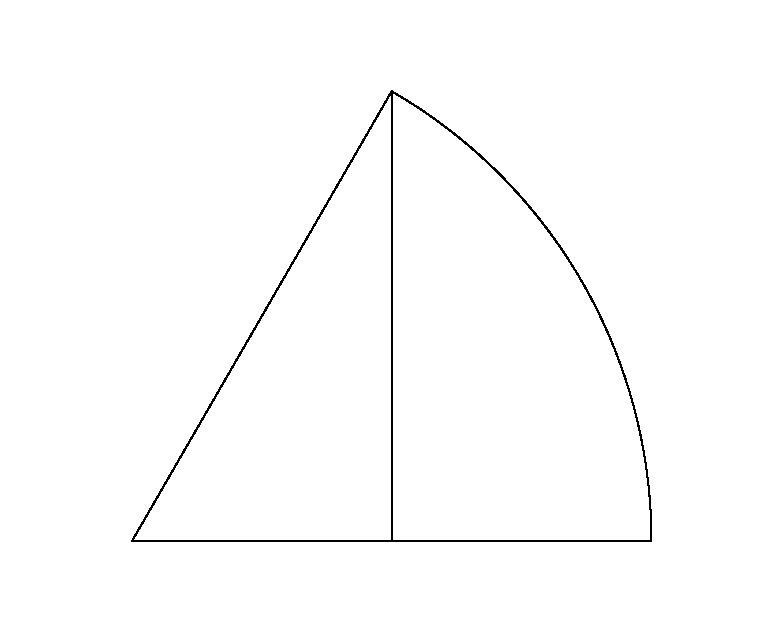
\includegraphics[scale=1]{circular_sector-inc}
\end{picture}%
\begin{picture}(360,288)(0,0)
\fontsize{12}{0}\selectfont\put(97.0695,158.213){\makebox(0,0)[l]{\textcolor[rgb]{0,0,0}{{$r$}}}}
\fontsize{12}{0}\selectfont\put(284.38,173.328){\makebox(0,0)[l]{\textcolor[rgb]{0,0,0}{{$s$}}}}
\fontsize{12}{0}\selectfont\put(113.905,14.1263){\makebox(0,0)[l]{\textcolor[rgb]{0,0,0}{{$x$}}}}
\fontsize{12}{0}\selectfont\put(199.33,143.498){\makebox(0,0)[l]{\textcolor[rgb]{0,0,0}{{$y$}}}}
\end{picture}
}
\caption{Circular sector.}
\end{figure}
\clearpage
\section{Circular Sector Sequence}
\subsection{Apothem}
\begin{equation}
\area \triangle ORS_{n-1} = \frac{\overline{RS_{n-1}} \overline{OX_n}}{2}, n \geq 1
\end{equation}
\begin{equation}
\area \triangle ORS_{n-1} = \frac{\overline{OS_{n-1}} \overline{RX_{n-1}}}{2}, n \geq 1
\end{equation}
\begin{equation}
\frac{\overline{RS_{n-1}} \overline{OX_n}}{2} = \frac{\overline{OS_{n-1}} \overline{RX_{n-1}}}{2}, n \geq 1
\end{equation}
\begin{equation}
\overline{RS_{n-1}} \overline{OX_n} = \overline{OS_{n-1}} \overline{RX_{n-1}}, n \geq 1
\end{equation}
\begin{equation}
\frac{\overline{RS_{n-1}} \overline{OX_n}}{\overline{RS_{n-1}}} = \frac{\overline{OS_{n-1}} \overline{RX_{n-1}}}{\overline{RS_{n-1}}}, n \geq 1
\end{equation}
\begin{equation}
\overline{OX_n} = \frac{\overline{OS_{n-1}} \overline{RX_{n-1}}}{\overline{RS_{n-1}}}, n \geq 1
\end{equation}
\begin{equation}
\overline{OX_n} = \frac{\overline{OS_{n-1}} \sqrt{\overline{OR}^2 - \overline{OX_{n-1}}^2}}{\overline{RS_{n-1}}}, n \geq 1
\end{equation}
\begin{equation}
\overline{OX_n} = \frac{\overline{OS_{n-1}} \sqrt{\overline{OR}^2 - \overline{OX_{n-1}}^2}}{\sqrt{\overline{OR}^2 + \overline{OS_{n-1}}^2 - 2 \overline{OS_{n-1}} \overline{OX_{n-1}}}}, n \geq 1
\end{equation}
\subsection{Chord Length}
\begin{equation}
\overline{RS_n} = \sqrt{\overline{RX_n}^2 + \overline{X_nS_n}^2}
\end{equation}
\begin{equation}
\overline{RS_n} = \sqrt{\left(\sqrt{\overline{OR}^2 - \overline{OX_n}^2}\right)^2 + \overline{X_nS_n}^2}
\end{equation}
\begin{equation}
\overline{RS_n} = \sqrt{\overline{OR}^2 - \overline{OX_n}^2 + \overline{X_nS_n}^2}
\end{equation}
\begin{equation}
\overline{RS_n} = \sqrt{\overline{OR}^2 - \overline{OX_n}^2 + \left(\overline{OS_n} - \overline{OX_n}\right)^2}
\end{equation}
\begin{equation}
\overline{RS_n} = \sqrt{\overline{OR}^2 - \overline{OX_n}^2 + \overline{OS_n}^2 - 2 \overline{OS_n} \overline{OX_n} + \overline{OX_n}^2}
\end{equation}
\begin{equation}
\overline{RS_n} = \sqrt{\overline{OR}^2 + \overline{OS_n}^2 - 2 \overline{OS_n} \overline{OX_n}}
\end{equation}
\subsection{Arc Length}
\begin{equation}
\arc RS_0 \stackrel{\text{def}}{=} \lim \limits_{n \to \infty} 2^n \overline{RS_n}
\end{equation}
\subsection{Area}
\begin{equation}
\area \sector ORS_0 = \lim \limits_{n \to \infty} 2^{n-1} \area ORS_nS_{n-1}
\end{equation}
\begin{equation}
\area \sector ORS_0 = \lim \limits_{n \to \infty} 2^{n-1} \frac{\overline{RS_{n-1}} \overline{OS_n}}{2}
\end{equation}
\begin{equation}
\area \sector ORS_0 = \frac{\lim \limits_{n \to \infty} 2^{n-1} \overline{RS_{n-1}} \overline{OS_n}}{2}
\end{equation}
\begin{equation}
\area \sector ORS_0 = \frac{\lim \limits_{n \to \infty} \left(2^{n-1} \overline{RS_{n-1}}\right) \overline{OS_n}}{2}
\end{equation}
\begin{equation}
\area \sector ORS_0 = \frac{\lim \limits_{n \to \infty} \overline{OS_n} \left(2^{n-1} \overline{RS_{n-1}}\right)}{2}
\end{equation}
\begin{equation}
\area \sector ORS_0 = \frac{\left(\lim \limits_{n \to \infty} \overline{OS_n}\right) \left(\lim \limits_{n \to \infty} 2^{n-1} \overline{RS_{n-1}}\right)}{2}
\end{equation}
\begin{equation}
\area \sector ORS_0 = \frac{\overline{OR} \lim \limits_{n \to \infty} 2^{n-1} \overline{RS_{n-1}}}{2}
\end{equation}
\begin{equation}
\area \sector ORS_0 = \frac{\overline{OR} \arc RS_0}{2}
\end{equation}
\clearpage
\begin{figure}[p]
\centering
\begin{subfigure}{\textwidth}
\centering
\resizebox{\textwidth}{!}{% Title: Figure 1
% Creator: GL2PS 1.4.2, (C) 1999-2020 C. Geuzaine
% For: Octave
% CreationDate: Fri Oct 16 07:42:27 2026
\setlength{\unitlength}{1pt}
\begin{picture}(0,0)
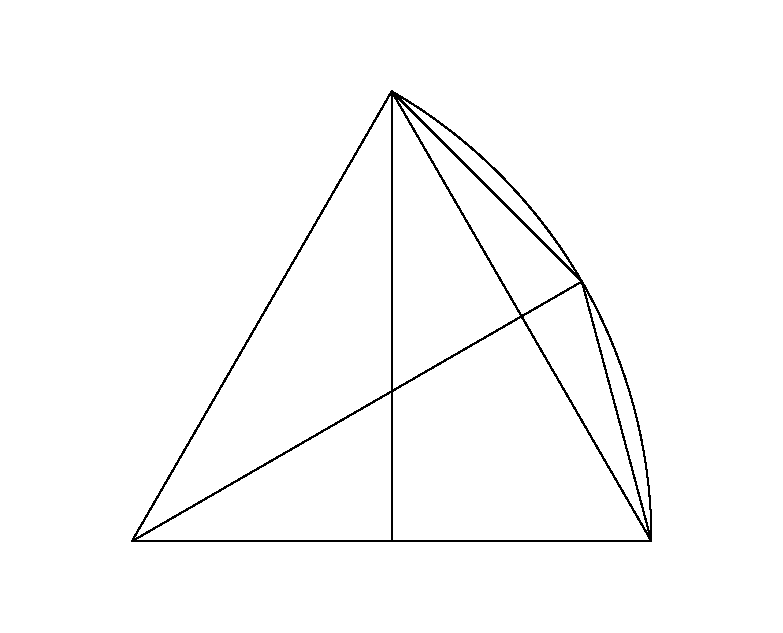
\includegraphics[scale=1]{circular_sector_sequence_recursive_step-inc}
\end{picture}%
\begin{picture}(360,288)(0,0)
\fontsize{12}{0}\selectfont\put(35.3393,14.1263){\makebox(0,0)[l]{\textcolor[rgb]{0,0,0}{{$O$}}}}
\fontsize{12}{0}\selectfont\put(176.259,274.69){\makebox(0,0)[l]{\textcolor[rgb]{0,0,0}{{$A$}}}}
\fontsize{12}{0}\selectfont\put(315.058,14.1263){\makebox(0,0)[l]{\textcolor[rgb]{0,0,0}{{$C_{n-1}$}}}}
\fontsize{12}{0}\selectfont\put(174.887,14.1263){\makebox(0,0)[l]{\textcolor[rgb]{0,0,0}{{$B_{n-1}$}}}}
\fontsize{12}{0}\selectfont\put(284.38,173.328){\makebox(0,0)[l]{\textcolor[rgb]{0,0,0}{{$C_n$}}}}
\fontsize{12}{0}\selectfont\put(227.139,111.598){\makebox(0,0)[l]{\textcolor[rgb]{0,0,0}{{$B_n$}}}}
\end{picture}
}
\caption{Recursive step.}
\end{subfigure}
\caption{Circular sector sequence.}
\end{figure}
\clearpage
\begin{figure}[p]
\centering
\ContinuedFloat
\begin{subfigure}{\textwidth}
\centering
\resizebox{\textwidth}{!}{% Title: Figure 1
% Creator: GL2PS 1.4.2, (C) 1999-2020 C. Geuzaine
% For: Octave
% CreationDate: Fri Oct 30 01:53:15 2026
\setlength{\unitlength}{1pt}
\begin{picture}(0,0)
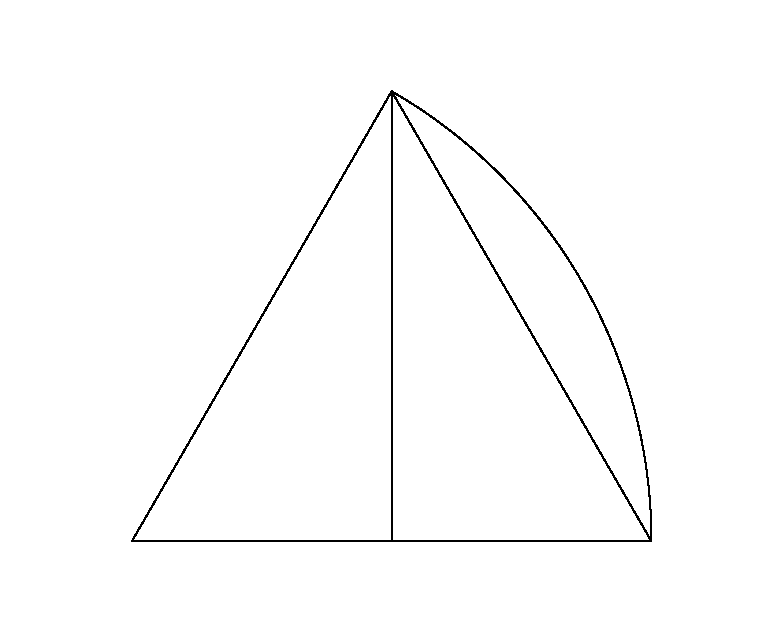
\includegraphics[scale=1]{circular_sector_sequence_base_case-inc}
\end{picture}%
\begin{picture}(360,288)(0,0)
\fontsize{12}{0}\selectfont\put(35.3393,14.1263){\makebox(0,0)[l]{\textcolor[rgb]{0,0,0}{{$O$}}}}
\fontsize{12}{0}\selectfont\put(176.259,274.69){\makebox(0,0)[l]{\textcolor[rgb]{0,0,0}{{$A$}}}}
\fontsize{12}{0}\selectfont\put(315.058,14.1263){\makebox(0,0)[l]{\textcolor[rgb]{0,0,0}{{$C_0$}}}}
\fontsize{12}{0}\selectfont\put(174.887,14.1263){\makebox(0,0)[l]{\textcolor[rgb]{0,0,0}{{$B_0$}}}}
\end{picture}
}
\caption{Base case.}
\end{subfigure}
\caption{Circular sector sequence.}
\end{figure}
\clearpage
\section{Simple Harmonic Motion}
\begin{equation}
[m] = \text{kg}
\end{equation}
\begin{equation}
[\omega] = \text{m/s}
\end{equation}
\begin{equation}
[k] = \text{N/m}
\end{equation}
\begin{equation}
[r] = \text{m}
\end{equation}
\begin{equation}
F = ma
\end{equation}
\begin{equation}
F = -kx
\end{equation}
\begin{equation}
ma = -kx
\end{equation}
\begin{equation}
s = \omega t
\end{equation}
\begin{equation}
\omega = \frac{\Delta s}{\Delta t}
\end{equation}
\begin{equation}
|x| \ll r \implies \omega \approx \left|\frac{\Delta x}{\Delta t}\right|
\end{equation}
\begin{equation}
x(t) = \cos(r,\omega t)
\end{equation}
\begin{equation}
v(t) = \left.\frac{\partial \cos(r,s)}{\partial s}\right|_{s = \omega t} \cdot \frac{d (\omega t)}{dt}
\end{equation}
\begin{equation}
v(t) = \frac{-\sin(r,\omega t)}{r} \cdot \frac{d (\omega t)}{dt}
\end{equation}
\begin{equation}
v(t) = \frac{-\sin(r,\omega t)}{r} \cdot \omega
\end{equation}
\begin{equation}
v(t) = \frac{-\omega \sin(r,\omega t)}{r}
\end{equation}
\begin{equation}
a(t) = \frac{dv}{dt}
\end{equation}
\begin{equation}
a(t) = \frac{d \left(\left.\frac{\partial \cos(r,s)}{\partial s}\right|_{s = \omega t} \frac{d (\omega t)}{dt}\right)}{dt}
\end{equation}
\begin{equation}
a(t) = \left(\left.\frac{\partial^2 \cos(r,s)}{\partial s^2} \cdot \frac{ds}{dt}\right|_{s = \omega t}\right) \cdot \frac{d (\omega t)}{dt} + \left.\frac{\partial \cos(r,s)}{\partial s}\right|_{s = \omega t} \cdot \frac{d^2 (\omega t)}{dt^2}
\end{equation}
\begin{equation}
a(t) = \left(\frac{-\cos(r,\omega t)}{r^2} \cdot \frac{d (\omega t)}{dt}\right) \cdot \frac{d (\omega t)}{dt} + \left.\frac{\partial \cos(r,s)}{\partial s}\right|_{s = \omega t} \cdot \frac{d^2 (\omega t)}{dt^2}
\end{equation}
\begin{equation}
a(t) = \frac{-\cos(r,\omega t)}{r^2} \cdot \left(\frac{d (\omega t)}{dt}\right)^2 + \left.\frac{\partial \cos(r,s)}{\partial s}\right|_{s = \omega t} \cdot \frac{d^2 (\omega t)}{dt^2}
\end{equation}
\begin{equation}
a(t) = \frac{-\cos(r,\omega t)}{r^2} \cdot \omega^2 + \left.\frac{\partial \cos(r,s)}{\partial s}\right|_{s = \omega t} \cdot \frac{d^2 (\omega t)}{dt^2}
\end{equation}
\begin{equation}
a(t) = \frac{-\omega^2 \cos(r,\omega t)}{r^2} + \left.\frac{\partial \cos(r,s)}{\partial s}\right|_{s = \omega t} \cdot \frac{d^2 (\omega t)}{dt^2}
\end{equation}
\begin{equation}
a(t) = \frac{-\omega^2 \cos(r,\omega t)}{r^2} + \frac{-\sin(r,\omega t)}{r} \cdot \frac{d^2 (\omega t)}{dt^2}
\end{equation}
\begin{equation}
a(t) = \frac{-\omega^2 \cos(r,\omega t)}{r^2} + \frac{-\sin(r,\omega t)}{r} \cdot 0
\end{equation}
\begin{equation}
a(t) = \frac{-\omega^2 \cos(r,\omega t)}{r^2} + 0
\end{equation}
\begin{equation}
a(t) = \frac{-\omega^2 \cos(r,\omega t)}{r^2}
\end{equation}
\begin{equation}
a(x) = \frac{-\omega^2 x}{r^2}
\end{equation}
\begin{equation}
m \frac{-\omega^2 x}{r^2} = -kx
\end{equation}
\begin{equation}
\frac{m (-\omega^2 x)}{r^2} = -kx
\end{equation}
\begin{equation}
\frac{-m \omega^2 x}{r^2} = -kx
\end{equation}
\begin{equation}
\frac{-m \omega^2 x}{r^2} = \frac{-kr^2x}{r^2}
\end{equation}
\begin{equation}
m \omega^2 = kr^2
\end{equation}
\begin{equation}
K(t) = \frac{mv^2(t)}{2}
\end{equation}
\begin{equation}
K(t) = \frac{m \left(\frac{-\omega \sin(r,\omega t)}{r}\right)^2}{2}
\end{equation}
\begin{equation}
K(t) = \frac{m \frac{(-\omega \sin(r,\omega t))^2}{r^2}}{2}
\end{equation}
\begin{equation}
K(t) = \frac{m \frac{(-\omega)^2 \sin^2(r,\omega t)}{r^2}}{2}
\end{equation}
\begin{equation}
K(t) = \frac{m \frac{\omega^2 \sin^2(r,\omega t)}{r^2}}{2}
\end{equation}
\begin{equation}
K(t) = \frac{\left(\frac{m \omega^2 \sin^2(r,\omega t)}{r^2}\right)}{2}
\end{equation}
\begin{equation}
K(t) = \frac{\left(\frac{kr^2 \sin^2(r,\omega t)}{r^2}\right)}{2}
\end{equation}
\begin{equation}
K(t) = \frac{k \sin^2(r,\omega t)}{2}
\end{equation}
\begin{equation}
U(t) = \frac{kx^2(t)}{2}
\end{equation}
\begin{equation}
U(t) = \frac{k \cos^2(r,\omega t)}{2}
\end{equation}
\begin{equation}
E = K + U
\end{equation}
\begin{equation}
E = \frac{k \sin^2(r,\omega t)}{2} + \frac{k \cos^2(r,\omega t)}{2}
\end{equation}
\begin{equation}
E = \frac{k \sin^2(r,\omega t) + k \cos^2(r,\omega t)}{2}
\end{equation}
\begin{equation}
E = \frac{k (\sin^2(r,\omega t) + \cos^2(r,\omega t))}{2}
\end{equation}
\begin{equation}
E = \frac{kr^2}{2}
\end{equation}
\begin{equation}
E = \frac{m \omega^2}{2}
\end{equation}
\clearpage
\begin{figure}[p]
\centering
\resizebox{\textwidth}{!}{% Title: Figure 1
% Creator: GL2PS 1.4.2, (C) 1999-2020 C. Geuzaine
% For: Octave
% CreationDate: Fri Oct 30 01:53:17 2026
\setlength{\unitlength}{1pt}
\begin{picture}(0,0)
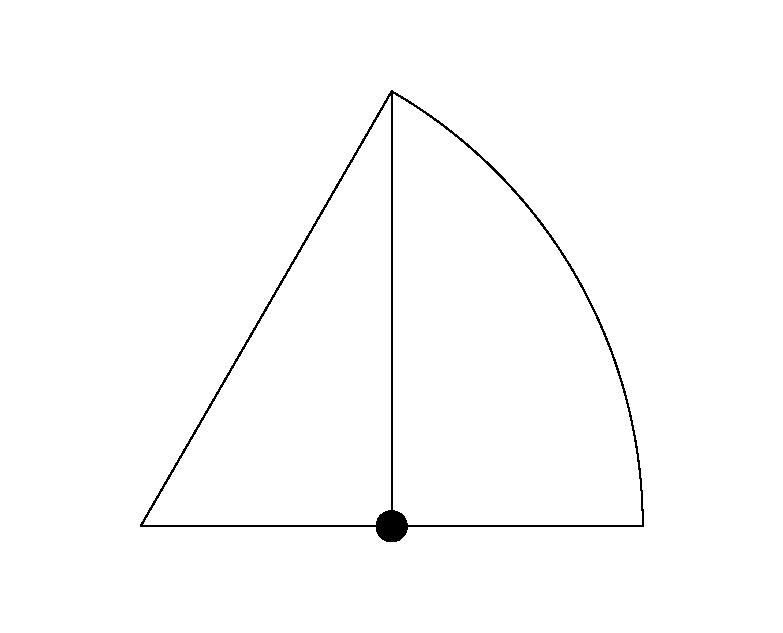
\includegraphics[scale=1]{simple_harmonic_motion-inc}
\end{picture}%
\begin{picture}(360,288)(0,0)
\fontsize{12}{0}\selectfont\put(99.8458,161.353){\makebox(0,0)[l]{\textcolor[rgb]{0,0,0}{{$r$}}}}
\fontsize{12}{0}\selectfont\put(280.886,175.962){\makebox(0,0)[l]{\textcolor[rgb]{0,0,0}{{$s$}}}}
\fontsize{12}{0}\selectfont\put(116.118,22.0896){\makebox(0,0)[l]{\textcolor[rgb]{0,0,0}{{$x$}}}}
\end{picture}
}
\caption{Simple harmonic motion.}
\end{figure}
\clearpage
\section{Uniform Circular Motion}
\begin{equation}
[m] = \text{kg}
\end{equation}
\begin{equation}
[\omega] = \text{m/s}
\end{equation}
\begin{equation}
[r] = \text{m}
\end{equation}
\begin{equation}
s = \omega t
\end{equation}
\begin{equation}
\omega = \frac{\Delta s}{\Delta t}
\end{equation}
\begin{equation}
x(t) = \cos(r,\omega t)
\end{equation}
\begin{equation}
y(t) = \sin(r,\omega t)
\end{equation}
\begin{equation}
\vec{r}(t) = (x,y)
\end{equation}
\begin{equation}
\vec{r}(t) = (\cos(r,\omega t),\sin(r,\omega t))
\end{equation}
\begin{equation}
\vec{v}(t) = \frac{d \vec{r}}{dt}
\end{equation}
\begin{equation}
\vec{v}(t) = \frac{d (x,y)}{dt}
\end{equation}
\begin{equation}
\vec{v}(t) = \left(\frac{dx}{dt},\frac{dy}{dt}\right)
\end{equation}
\begin{equation}
\frac{dx}{dt} = \left.\frac{\partial \cos(r,s)}{\partial s}\right|_{s = \omega t} \cdot \frac{d (\omega t)}{dt}
\end{equation}
\begin{equation}
\frac{dx}{dt} = \frac{-\sin(r,\omega t)}{r} \cdot \frac{d (\omega t)}{dt}
\end{equation}
\begin{equation}
\frac{dx}{dt} = \frac{-\sin(r,\omega t)}{r} \cdot \omega
\end{equation}
\begin{equation}
\frac{dx}{dt} = \frac{-\omega \sin(r,\omega t)}{r}
\end{equation}
\begin{equation}
\frac{dy}{dt} = \left.\frac{\partial \sin(r,s)}{\partial s}\right|_{s = \omega t} \cdot \frac{d (\omega t)}{dt}
\end{equation}
\begin{equation}
\frac{dy}{dt} = \frac{\cos(r,\omega t)}{r} \cdot \frac{d (\omega t)}{dt}
\end{equation}
\begin{equation}
\frac{dy}{dt} = \frac{\cos(r,\omega t)}{r} \cdot \omega
\end{equation}
\begin{equation}
\frac{dy}{dt} = \frac{\omega \cos(r,\omega t)}{r}
\end{equation}
\begin{equation}
\vec{v}(t) = \left(\frac{-\omega \sin(r,\omega t)}{r},\frac{\omega \cos(r,\omega t)}{r}\right)
\end{equation}
\begin{equation}
\vec{v}(t) = \frac{\omega \left(-\sin(r,\omega t),\cos(r,\omega t)\right)}{r}
\end{equation}
\begin{equation}
v = \left|\vec{v}\right|
\end{equation}
\begin{equation}
v = \left|\frac{\omega \left(-\sin(r,\omega t),\cos(r,\omega t)\right)}{r}\right|
\end{equation}
\begin{equation}
v = \frac{\left|\omega \left(-\sin(r,\omega t),\cos(r,\omega t)\right)\right|}{\left|r\right|}
\end{equation}
\begin{equation}
v = \frac{\left|\omega\right| \left|\left(-\sin(r,\omega t),\cos(r,\omega t)\right)\right|}{\left|r\right|}
\end{equation}
\begin{equation}
v = \frac{\omega \left|\left(-\sin(r,\omega t),\cos(r,\omega t)\right)\right|}{\left|r\right|}
\end{equation}
\begin{equation}
v = \frac{\omega \sqrt{(-\sin(r,\omega t))^2 + \cos^2(r,\omega t)}}{\left|r\right|}
\end{equation}
\begin{equation}
v = \frac{\omega \sqrt{\sin^2(r,\omega t) + \cos^2(r,\omega t)}}{\left|r\right|}
\end{equation}
\begin{equation}
v = \frac{\omega \sqrt{r^2}}{\left|r\right|}
\end{equation}
\begin{equation}
v = \frac{\omega \left|r\right|}{\left|r\right|}
\end{equation}
\begin{equation}
v = \omega
\end{equation}
\begin{equation}
E = \frac{mv^2}{2}
\end{equation}
\begin{equation}
E = \frac{m \omega^2}{2}
\end{equation}
\begin{equation}
\vec{a}(t) = \frac{d^2 \vec{r}}{dt^2}
\end{equation}
\begin{equation}
\vec{a}(t) = \frac{d^2 (x,y)}{dt^2}
\end{equation}
\begin{equation}
\vec{a}(t) = \left(\frac{d^2x}{dt^2},\frac{d^2y}{dt^2}\right)
\end{equation}
\begin{equation}
\frac{d^2x}{dt^2} = \frac{d \left(\left.\frac{\partial \cos(r,s)}{\partial s}\right|_{s = \omega t} \frac{d (\omega t)}{dt}\right)}{dt}
\end{equation}
\begin{equation}
\frac{d^2x}{dt^2} = \left(\left.\frac{\partial^2 \cos(r,s)}{\partial s^2} \cdot \frac{ds}{dt}\right|_{s = \omega t}\right) \cdot \frac{d (\omega t)}{dt} + \left.\frac{\partial \cos(r,s)}{\partial s}\right|_{s = \omega t} \cdot \frac{d^2 (\omega t)}{dt^2}
\end{equation}
\begin{equation}
\frac{d^2x}{dt^2} = \left(\frac{-\cos(r,\omega t)}{r^2} \cdot \frac{d (\omega t)}{dt}\right) \cdot \frac{d (\omega t)}{dt} + \left.\frac{\partial \cos(r,s)}{\partial s}\right|_{s = \omega t} \cdot \frac{d^2 (\omega t)}{dt^2}
\end{equation}
\begin{equation}
\frac{d^2x}{dt^2} = \frac{-\cos(r,\omega t)}{r^2} \cdot \left(\frac{d (\omega t)}{dt}\right)^2 + \left.\frac{\partial \cos(r,s)}{\partial s}\right|_{s = \omega t} \cdot \frac{d^2 (\omega t)}{dt^2}
\end{equation}
\begin{equation}
\frac{d^2x}{dt^2} = \frac{-\cos(r,\omega t)}{r^2} \cdot \omega^2 + \left.\frac{\partial \cos(r,s)}{\partial s}\right|_{s = \omega t} \cdot \frac{d^2 (\omega t)}{dt^2}
\end{equation}
\begin{equation}
\frac{d^2x}{dt^2} = \frac{-\omega^2 \cos(r,\omega t)}{r^2} + \left.\frac{\partial \cos(r,s)}{\partial s}\right|_{s = \omega t} \cdot \frac{d^2 (\omega t)}{dt^2}
\end{equation}
\begin{equation}
\frac{d^2x}{dt^2} = \frac{-\omega^2 \cos(r,\omega t)}{r^2} + \frac{-\sin(r,\omega t)}{r} \cdot \frac{d^2 (\omega t)}{dt^2}
\end{equation}
\begin{equation}
\frac{d^2x}{dt^2} = \frac{-\omega^2 \cos(r,\omega t)}{r^2} + \frac{-\sin(r,\omega t)}{r} \cdot 0
\end{equation}
\begin{equation}
\frac{d^2x}{dt^2} = \frac{-\omega^2 \cos(r,\omega t)}{r^2} + 0
\end{equation}
\begin{equation}
\frac{d^2x}{dt^2} = \frac{-\omega^2 \cos(r,\omega t)}{r^2}
\end{equation}
\begin{equation}
\frac{d^2y}{dt^2} = \frac{d \left(\left.\frac{\partial \sin(r,s)}{\partial s}\right|_{s = \omega t} \frac{d (\omega t)}{dt}\right)}{dt}
\end{equation}
\begin{equation}
\frac{d^2y}{dt^2} = \left(\left.\frac{\partial^2 \sin(r,s)}{\partial s^2} \cdot \frac{ds}{dt}\right|_{s = \omega t}\right) \cdot \frac{d (\omega t)}{dt} + \left.\frac{\partial \sin(r,s)}{\partial s}\right|_{s = \omega t} \cdot \frac{d^2 (\omega t)}{dt^2}
\end{equation}
\begin{equation}
\frac{d^2y}{dt^2} = \left(\frac{-\sin(r,\omega t)}{r^2} \cdot \frac{d (\omega t)}{dt}\right) \cdot \frac{d (\omega t)}{dt} + \left.\frac{\partial \sin(r,s)}{\partial s}\right|_{s = \omega t} \cdot \frac{d^2 (\omega t)}{dt^2}
\end{equation}
\begin{equation}
\frac{d^2y}{dt^2} = \frac{-\sin(r,\omega t)}{r^2} \cdot \left(\frac{d (\omega t)}{dt}\right)^2 + \left.\frac{\partial \sin(r,s)}{\partial s}\right|_{s = \omega t} \cdot \frac{d^2 (\omega t)}{dt^2}
\end{equation}
\begin{equation}
\frac{d^2y}{dt^2} = \frac{-\sin(r,\omega t)}{r^2} \cdot \omega^2 + \left.\frac{\partial \sin(r,s)}{\partial s}\right|_{s = \omega t} \cdot \frac{d^2 (\omega t)}{dt^2}
\end{equation}
\begin{equation}
\frac{d^2y}{dt^2} = \frac{-\omega^2 \sin(r,\omega t)}{r^2} + \left.\frac{\partial \sin(r,s)}{\partial s}\right|_{s = \omega t} \cdot \frac{d^2 (\omega t)}{dt^2}
\end{equation}
\begin{equation}
\frac{d^2y}{dt^2} = \frac{-\omega^2 \sin(r,\omega t)}{r^2} + \frac{\cos(r,\omega t)}{r} \cdot \frac{d^2 (\omega t)}{dt^2}
\end{equation}
\begin{equation}
\frac{d^2y}{dt^2} = \frac{-\omega^2 \sin(r,\omega t)}{r^2} + \frac{\cos(r,\omega t)}{r} \cdot 0
\end{equation}
\begin{equation}
\frac{d^2y}{dt^2} = \frac{-\omega^2 \sin(r,\omega t)}{r^2} + 0
\end{equation}
\begin{equation}
\frac{d^2y}{dt^2} = \frac{-\omega^2 \sin(r,\omega t)}{r^2}
\end{equation}
\begin{equation}
\vec{a}(t) = \left(\frac{-\omega^2 \cos(r,\omega t)}{r^2},\frac{-\omega^2 \sin(r,\omega t)}{r^2}\right)
\end{equation}
\begin{equation}
\vec{a}(t) = \frac{-\omega^2 \left(\cos(r,\omega t),\sin(r,\omega t)\right)}{r^2}
\end{equation}
\begin{equation}
\vec{a} = \frac{-\omega^2 \vec{r}}{r^2}
\end{equation}
\begin{equation}
a = \left|\vec{a}\right|
\end{equation}
\begin{equation}
a = \left|\frac{-\omega^2 \vec{r}}{r^2}\right|
\end{equation}
\begin{equation}
a = \frac{\left|-\omega^2 \vec{r}\right|}{\left|r^2\right|}
\end{equation}
\begin{equation}
a = \frac{\left|-\omega^2\right| \left|\vec{r}\right|}{\left|r^2\right|}
\end{equation}
\begin{equation}
a = \frac{\omega^2 \left|\vec{r}\right|}{\left|r^2\right|}
\end{equation}
\begin{equation}
a = \frac{\omega^2 r}{\left|r^2\right|}
\end{equation}
\begin{equation}
a = \frac{\omega^2 r}{r^2}
\end{equation}
\begin{equation}
a = \frac{\omega^2}{r}
\end{equation}
\begin{equation}
F = ma
\end{equation}
\begin{equation}
F = m \frac{\omega^2}{r}
\end{equation}
\begin{equation}
F = \frac{m \omega^2}{r}
\end{equation}
\clearpage
\begin{figure}[p]
\centering
\resizebox{\textwidth}{!}{% Title: Figure 1
% Creator: GL2PS 1.4.2, (C) 1999-2020 C. Geuzaine
% For: Octave
% CreationDate: Tue Oct 20 09:35:33 2026
\setlength{\unitlength}{1pt}
\begin{picture}(0,0)
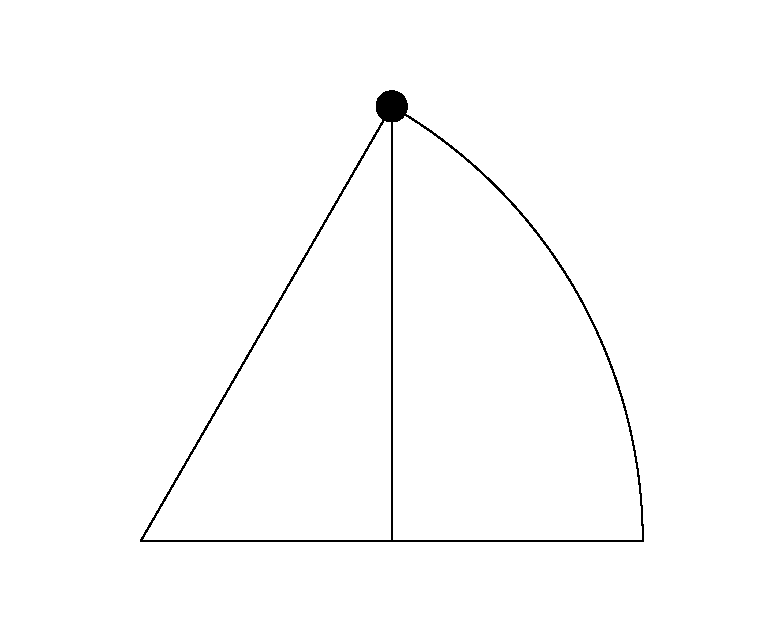
\includegraphics[scale=1]{uniform_circular_motion-inc}
\end{picture}%
\begin{picture}(360,288)(0,0)
\fontsize{12}{0}\selectfont\put(99.8461,154.121){\makebox(0,0)[l]{\textcolor[rgb]{0,0,0}{{$r$}}}}
\fontsize{12}{0}\selectfont\put(280.885,168.73){\makebox(0,0)[l]{\textcolor[rgb]{0,0,0}{{$s$}}}}
\fontsize{12}{0}\selectfont\put(116.118,14.8587){\makebox(0,0)[l]{\textcolor[rgb]{0,0,0}{{$x$}}}}
\fontsize{12}{0}\selectfont\put(198.682,139.899){\makebox(0,0)[l]{\textcolor[rgb]{0,0,0}{{$y$}}}}
\end{picture}
}
\caption{Uniform circular motion.}
\end{figure}
\clearpage
\begin{figure}[p]
\centering
\resizebox{\textwidth}{!}{% Title: Figure 1
% Creator: GL2PS 1.4.2, (C) 1999-2020 C. Geuzaine
% For: Octave
% CreationDate: Wed Oct 28 07:46:53 2026
\setlength{\unitlength}{1pt}
\begin{picture}(0,0)
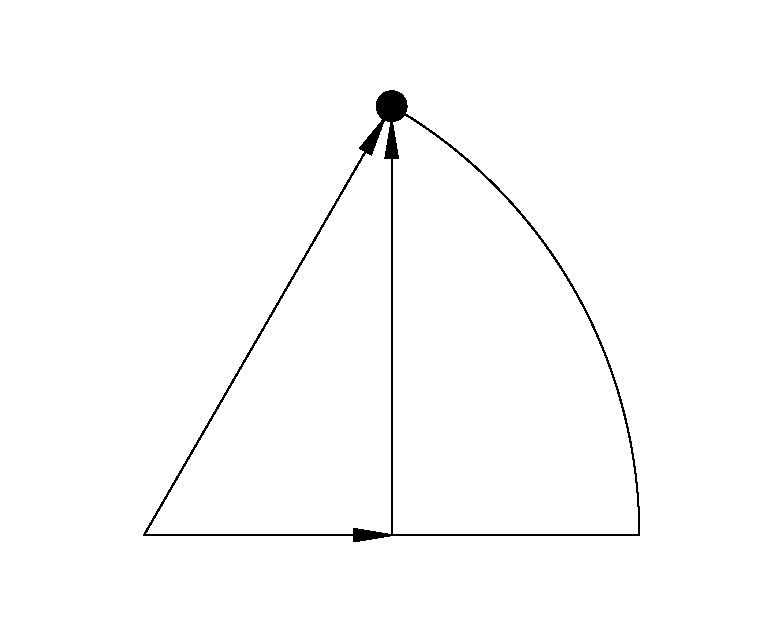
\includegraphics[scale=1]{uniform_circular_motion_position_vector_diagram-inc}
\end{picture}%
\begin{picture}(360,288)(0,0)
\fontsize{12}{0}\selectfont\put(100.949,155.468){\makebox(0,0)[l]{\textcolor[rgb]{0,0,0}{{$\vec{r}$}}}}
\fontsize{12}{0}\selectfont\put(116.997,18.1214){\makebox(0,0)[l]{\textcolor[rgb]{0,0,0}{{$\vec{r}_x$}}}}
\fontsize{12}{0}\selectfont\put(198.425,141.441){\makebox(0,0)[l]{\textcolor[rgb]{0,0,0}{{$\vec{r}_y$}}}}
\end{picture}
}
\caption{Uniform circular motion (vector diagram).}
\end{figure}
\end{document}
